\UseRawInputEncoding


%%%%%%%%%%%%%%%%%%%%%%%%%%%%%%%%%%%%%%%%%%%%%%%%%%%%%%%%%%%%%%%%%%%%%%%%%%%%%%%%
%% Settings
%%%%%%%%%%%%%%%%%%%%%%%%%%%%%%%%%%%%%%%%%%%%%%%%%%%%%%%%%%%%%%%%%%%%%%%%%%%%%%%%
\documentclass[final,3p,times,twocolumn]{elsarticle}
%% Use the options 1p,twocolumn; 3p; 3p,twocolumn; 5p; or 5p,twocolumn
%% for a journal layout:
%% \documentclass[final,1p,times]{elsarticle}
%% \documentclass[final,1p,times,twocolumn]{elsarticle}
%% \documentclass[final,3p,times]{elsarticle}
%% \documentclass[final,3p,times,twocolumn]{elsarticle}
%% \documentclass[final,5p,times]{elsarticle}
%% \documentclass[final,5p,times,twocolumn]{elsarticle}
%% \documentclass[preprint,review,12pt]{elsarticle}

%% Image width
\newlength{\imagewidth}
\newlength{\imagescale}
%% preamble
\usepackage[english]{babel}
\usepackage[table]{xcolor} % For coloring tables
\usepackage{booktabs} % For professional quality tables
\usepackage{colortbl} % For coloring cells in tables
\usepackage{amsmath, amssymb} % For mathematical symbols and environments
\usepackage{amsthm} % For theorem-like environments
\usepackage{lipsum} % just for sample text
\usepackage{natbib}
\usepackage{graphicx}
\usepackage{indentfirst}
\usepackage{bashful}
% for figures
\usepackage[margin=10pt,font=small,labelfont=bf,labelsep=endash]{caption}
\usepackage{graphicx}
\usepackage{calc}
% for tables
% \usepackage{xlsx2csv}
% \usepackage{csv2latex}
\usepackage[T1]{fontenc} % [REVISED]
\usepackage[utf8]{inputenc} % [REVISED]
\usepackage{hyperref}
\usepackage{accsupp}

%% Line numbers
% \linenumbers

%% Tables
\usepackage{pdflscape}
\usepackage{csvsimple}
\usepackage{xltabular}
\usepackage{booktabs}
\usepackage{siunitx}
\usepackage{makecell}
\sisetup{round-mode=figures,round-precision=3}
\renewcommand\theadfont{\bfseries}
\renewcommand\theadalign{c}

\newcolumntype{C}[1]{>{\centering\arraybackslash}m{#1}}

%% Diff
% Define commands for highlighting
% diff
\usepackage[most]{tcolorbox} % for boxes with transparency
% Define colors with transparency (opacity value)
\definecolor{GreenBG}{rgb}{0,1,0}
\definecolor{RedBG}{rgb}{1,0,0}

% Define tcolorbox environments for highlighting
\newtcbox{\greenhighlight}[1][]{%
  on line,
  colframe=GreenBG,
  colback=GreenBG!50!white, % 50% transparent green
  boxrule=0pt,
  arc=0pt,
  boxsep=0pt,
  left=1pt,
  right=1pt,
  top=2pt,
  bottom=2pt,
  tcbox raise base
}

\newtcbox{\redhighlight}[1][]{%
  on line,
  colframe=RedBG,
  colback=RedBG!50!white, % 50% transparent red
  boxrule=0pt,
  arc=0pt,
  boxsep=0pt,
  left=1pt,
  right=1pt,
  top=2pt,
  bottom=2pt,
  tcbox raise base
}

\newcommand{\REDSTARTS}{\color{red}}
\newcommand{\REDENDS}{\color{black}}
\newcommand{\GREENSTARTS}{\color{green}}
\newcommand{\GREENENDS}{\color{black}}

% % Uncomment or provide the original definitions for these commands
% \newcommand{\REDSTARTS}{\color{red}}
% \newcommand{\REDENDS}{\color{black}} % Switch back to the default text color
% \newcommand{\GREENSTARTS}{\color{green}}
% \newcommand{\GREENENDS}{\color{black}} % Switch back to the default text color

% % Redefine the highlighting commands to use the tcolorbox environments
% \renewcommand{\REDSTARTS}{\begingroup\colorlet{oldcolor}{.}\color{red}}
% \renewcommand{\REDENDS}{\color{oldcolor}\endgroup}
% \renewcommand{\GREENSTARTS}{\begingroup\colorlet{oldcolor}{.}\color{green}}
% \renewcommand{\GREENENDS}{\color{oldcolor}\endgroup}

% % Define a command to apply the tcolorbox highlighting
% \newcommand{\highlight}[2]{\tcbox[colframe=#1,colback=#1!50!white,on line]{#2}}

% % Use the new \highlight command within the redefined \REDSTARTS and \GREENSTARTS
% \renewcommand{\REDSTARTS}{\highlight{RedBG}}
% \renewcommand{\GREENSTARTS}{\highlight{GreenBG}}
\GREENENDS \REDSTARTS s}\REDENDS 

%%%%%%%%%%%%%%%%%%%%%%%%%%%%%%%%%%%%%%%%%%%%%%%%%%%%%%%%%%%%%%%%%%%%%%%%%%%%%%%%
%% Journal Name
%%%%%%%%%%%%%%%%%%%%%%%%%%%%%%%%%%%%%%%%%%%%%%%%%%%%%%%%%%%%%%%%%%%%%%%%%%%%%%%%
\\REDSTARTS input{./src/\REDENDS journal\GREENSTARTS {Heliyon}\GREENENDS \REDSTARTS _name}
\REDENDS 
%%%%%%%%%%%%%%%%%%%%%%%%%%%%%%%%%%%%%%%%%%%%%%%%%%%%%%%%%%%%%%%%%%%%%%%%%%%%%%%%
%% Document Starts
%%%%%%%%%%%%%%%%%%%%%%%%%%%%%%%%%%%%%%%%%%%%%%%%%%%%%%%%%%%%%%%%%%%%%%%%%%%%%%%%
\begin{document}


%%%%%%%%%%%%%%%%%%%%%%%%%%%%%%%%%%%%%%%%%%%%%%%%%%%%%%%%%%%%%%%%%%%%%%%%%%%%%%%%
%% frontmatter
%%%%%%%%%%%%%%%%%%%%%%%%%%%%%%%%%%%%%%%%%%%%%%%%%%%%%%%%%%%%%%%%%%%%%%%%%%%%%%%%
\begin{frontmatter}
\GREENSTARTS \begin{highlights}\GREENENDS \REDSTARTS 	\begin{highlights}
\pdfbookmark[1]{Highlights}{highlights}

\item Neural trajectories in the hippocampus exhibited greater variability during a working memory (WM) task compared to those in the entorhinal cortex and amygdala regions.

\item The distance of neural trajectories between encoding and retrieval states in the hippocampus was memory-load dependent during a WM task.


\item Hippocampal neural trajectories fluctuated between the encoding and retrieval states in a task-dependent manner during both baseline and sharp-wave ripple (SWR) periods.

\item Hippocampal neural trajectories shifted from encoding to retrieval states during SWR period.

\end{highlights}
	\title{
Hippocampal neural fluctuations between memory encoding and retrieval states during a working memory task in humans: Encoding-to-retrieval shift during sharp-wave ripples
}
	\author[1]{Yusuke Watanabe\corref{cor1}}
\author[2,3,4]{Yuji Ikegaya}
\author[1,5]{Takufumi Yanagisawa}

\address[1]{Institute for Advanced Cocreation studies, Osaka University, 2-2 Yamadaoka, Suita, 565-0871, Osaka, Japan}
\address[2]{Graduate School of Pharmaceutical Sciences, The University of Tokyo, 7-3-1 Hongo, Tokyo, 113-0033, Japan}
\address[3]{Institute for AI and Beyond, The University of Tokyo, 7-3-1 Hongo, Tokyo, 113-0033, Japan}
\address[4]{Center for Information and Neural Networks, National Institute of Information and Communications Technology, 1-4 Yamadaoka, Suita City, 565-0871, Osaka, Japan}
\address[5]{Department of Neurosurgery, Osaka University Graduate School of Medicine, 2-2 Yamadaoka, Osaka, 565-0871, Japan}

\cortext[cor1]{Corresponding author. Tel: +81-6-6879-3652}
	%%Graphical abstract
%\pdfbookmark[1]{Graphical Abstract}{graphicalabstract}        
%\begin{graphicalabstract}
%\includegraphics{grabs}
%\end{graphicalabstract}

	\begin{abstract}
\pdfbookmark[1]{Abstract}{abstract}
Working memory (WM) plays a pivotal role in multiple cognitive functions, yet the complex neural mechanisms supporting its operation continue to remain unclear. In particular, despite the recognized roles of the hippocampus and sharp-wave ripple complexes (SWRs) -- brief, synchronous neural oscillations observed in the hippocampus -- in memory consolidation and retrieval, their contribution to WM tasks remains undefined. We demonstrate that during a WM task, multiunit activity patterns in the hippocampus exhibit unique dynamics, particularly during SWR periods. This study analyzed a dataset obtained from intracranial electroencephalogram recordings performed in the medial temporal lobe (MTL) of nine epilepsy patients during an eight-second Sternberg task. We employed Gaussian-process factor analysis to identify low-dimensional neural representations, referred to as 'trajectories,' within the MTL regions during the WM task. The results depicted significant variations in hippocampal neural trajectories as opposed to those in the entorhinal cortex and amygdala. Moreover, the trajectory distance between the encoding and retrieval phases was memory load-dependent. Notably, hippocampal trajectories during the retrieval phase showcased oscillations between encoding and retrieval states, contingent on the task type, particularly displaying a transient shift from encoding to retrieval states during SWRs. These findings emphasize the hippocampus's central role in executing WM tasks and suggest a future research hypothesis: the functional state of the hippocampus transitions from encoding to retrieval during SWRs.
\end{abstract}
	% \pdfbookmark[1]{Keywords}{keywords}                
\begin{keyword}
working memory \sep memory load \sep hippocampus \sep sharp-wave ripples \sep humans
\end{keyword}

\end{frontmatter}

%%%%%%%%%%%%%%%%%%%%%%%%%%%%%%%%%%%%%%%%%%%%%%%%%%%%%%%%%%%%%%%%%%%%%%%%%%%%%%%%
%% IMRaD
%%%%%%%%%%%%%%%%%%%%%%%%%%%%%%%%%%%%%%%%%%%%%%%%%%%%%%%%%%%%%%%%%%%%%%%%%%%%%%%%
\section{Introduction}
Working memory (WM) plays a crucial role in everyday life, and its neural underpinnings remain an area of ongoing research. The hippocampus, notably integral to memory, continues to be a primary focus of this investigation \cite{scoville_loss_1957} \cite{squire_legacy_2009}  \cite{boran_persistent_2019} \cite{kaminski_persistently_2017} \cite{kornblith_persistent_2017} \cite{faraut_dataset_2018} \cite{borders_hippocampus_2022} \cite{li_functional_2023} \cite{dimakopoulos_information_2022}. Gaining insights into the role of the hippocampus in working memory is vital to deepening our understanding of cognitive processes, hence fostering the progression of cognitive training and interventions.
\\
\indent
Current evidence suggests a transient, synchronized oscillation, referred to as sharp-wave ripple (SWR) \cite{buzsaki_hippocampal_2015}, is linked with several cognitive functions, such as memory replay \cite{wilson_reactivation_1994} \cite{nadasdy_replay_1999} \cite{lee_memory_2002} \cite{diba_forward_2007} \cite{davidson_hippocampal_2009}, memory consolidation \cite{girardeau_selective_2009} \cite{ego-stengel_disruption_2010} \cite{fernandez-ruiz_long-duration_2019} \cite{kim_corticalhippocampal_2022}, memory recall \cite{wu_hippocampal_2017} \cite{norman_hippocampal_2019} \cite{norman_hippocampal_2021}, and neural plasticity \cite{behrens_induction_2005} \cite{norimoto_hippocampal_2018}. This evidence indicates the likelihood that SWR could be a critical component of hippocampal processing, contributing to working memory performance. However, research investigating the effects of SWRs on working memory remains sparse \cite{jadhav_awake_2012}, and is largely limited to rodent models participating in navigation tasks where the timing of memory acquisition and recall is not explicitly distinguished.
\\
\indent
Recent studies indicate that hippocampal neurons exhibit low-dimensional representations during WM tasks. Notably, the firing patterns of place cells \cite{okeefe_hippocampus_1971} \cite{okeefe_place_1976} \cite{ekstrom_cellular_2003} \cite{kjelstrup_finite_2008} \cite{harvey_intracellular_2009}, located in the hippocampus, are observed to be encompassed within a dynamic, nonlinear three-dimensional hyperbolic geometry in rodents \cite{zhang_hippocampal_2022}. Moreover, grid cells in the entorhinal cortex (EC)—the dominant pathway to the hippocampus \cite{naber_reciprocal_2001} \cite{van_strien_anatomy_2009} \cite{strange_functional_2014}—displayed toroidal topology during exploration \cite{gardner_toroidal_2022}. Unfortunately, these investigations are confined to spatial navigation tasks in rodents, thus imposing limitations on the temporal resolution of WM tasks. The applicability of these findings to human subjects and their generalization beyond navigation tasks remains to be established.
\\
\indent
Given these considerations, the current study aims to validate the hypothesis that hippocampal neurons exhibit distinctive representations in low-dimensional spaces, designated as 'neural trajectory,' during WM tasks, most prominently within SWR periods. To evaluate this claim, we employed a dataset of patients performing an eight-second Sternberg task with high temporal resolution (1 s for fixation, 2 s for encoding, 3 s for maintenance, and 2 s for retrieval), while their intracranial electroencephalography signals (iEEG) within the medial temporal lobe (MTL) were being monitored \cite{boran_dataset_2020}. To investigate low-dimensional neural trajectories, we employed Gaussian-process factor analysis (GPFA), a method renowned for analyzing neural population dynamics \cite{yu_gaussian-process_2009}.
\label{sec:introduction}
\section{Methods}
\subsection{Dataset}
The dataset used in this study, which is publicly available, comprises nine epilepsy patients performing a modified Sternberg task \cite{boran_dataset_2020}. This task includes four phases: fixation (1s), encoding (2s), maintenance (3s), and retrieval (2s). During the encoding phase, participants were presented with a set of four, six, or eight alphabet letters. They were then tasked with determining whether a probe letter displayed during the retrieval phase had previously appeared (the correct response for Match IN task) or not (the correct response for Mismatch OUT task). Intracranial electroencephalography (iEEG) signals were captured with a 32 kHz sampling rate within a 0.5--5,000 Hz frequency range, using depth electrodes in medial temporal lobe (MTL) regions: the anterior head of the left and right hippocampus (AHL and AHR), the posterior body of the hippocampus (PHL and PHR), the entorhinal cortex (ECL and ECR), and the amygdala (AL and AR), as depicted in Figure~\ref{fig:01}A and Table~\ref{tab:01}. The iEEG signals were subsequently downsampled to 2 kHz. Correlations between variables such as set size and correct rate were examined (Figure~\ref{fig:s01}S1). Multiunit spike timings were determined via a spike sorting algorithm \cite{niediek_reliable_2016} using the Combinato package (\url{https://github.com/jniediek/combinato})(Figure~\ref{fig:01}C).

\subsection{Calculation of neural trajectories using GPFA}
Neural trajectories, also referred to as 'factors', in the hippocampus, EC, and amygdala were determined using GPFA \cite{yu_gaussian-process_2009} applied to the multiunit activity data for each session, performed with the elephant package (\url{https://elephant.readthedocs.io/en/latest/reference/gpfa.html}). The bin size was set to 50 ms, without overlaps. Each factor was z-normalized across all sessions, and the Euclidean distance from the origin ($O$) was then computed.
\\
\indent
For each trajectory within a region such as AHL, geometric medians ($\mathrm{g_{F}}$ for fixation, $\mathrm{g_{E}}$ for encoding, $\mathrm{g_{M}}$ for maintenance, and $\mathrm{g_{R}}$ for retrieval phase) were calculated by determining the median coordinates of the trajectory during the four phases. An optimal GPFA dimensionality was found to be three using the elbow method obtained by examining the log-likelihood values through a three-fold cross-validation approach (Figure~\ref{fig:02}B).

\subsection{Identifying SWR candidates from hippocampal regions}
Potential SWR events within the hippocampus were detected using a widely used method \cite{liu_consensus_2022}. LFP signals from a region of interest (ROI) like AHL, were re-referenced by deducting the averaged signal from locations outside the ROI (for instance, AHR, PHL, PHR, ECL, ECR, AL, and AR). The re-referenced LFP signals were then filtered with a ripple-band filter (80--140 Hz) to determine SWR candidates, marked as $\textrm{SWR}^+$ candidates. SWR detection was carried out using a published tool (\url{https://github.com/Eden-Kramer-Lab/ripple_detection}) \cite{kay_hippocampal_2016}, with the bandpass range adjusted to 80--140 Hz for humans \cite{norman_hippocampal_2019} \cite{norman_hippocampal_2021}, unlike the initial 150--250 Hz range typically applied to rodents.
\\
\indent
Control events for $\textrm{SWR}^+$ candidates, labeled as $\textrm{SWR}^-$ candidates, were detected by randomly shuffling the timestamps of $\textrm{SWR}^+$ candidates across all trials and subjects. The resulting $\textrm{SWR}^+/\textrm{SWR}^-$ candidates were then visually inspected.

\subsection{Defining SWRs from putative hippocampal CA1 regions}
Potential SWRs were differentiated from SWR candidates in putative CA1 (cornu Ammonis 1) regions. These regions were initially defined as follows: $\textrm{SWR}^+/\textrm{SWR}^-$ candidates in the hippocampus were projected into a two-dimensional space based on overlapping spike counts per unit using a supervised method, UMAP (Uniform Manifold Approximation and Projection) \cite{mcinnes_umap_2018}. Clustering validation was performed by calculating the silhouette score \cite{rousseeuw_silhouettes_1987} from clustered samples. Regions in the hippocampus, which scored above 0.6 on average across sessions (75th percentile), were identified as putative CA1 regions, resulting in the identification of five electrode positions from five patients.
\\
\indent
$\textrm{SWR}^+/\textrm{SWR}^-$ candidates in these predetermined CA1 regions were categorized as $\textrm{SWR}^+/\textrm{SWR}^-$, and thus they no longer retained their candidate status. The duration and ripple band peak amplitude of SWRs were found to follow log-normal distributions. Each time period of SWR was partitioned relative to the time from the SWR center into pre- (at $-800$ to $-300$ ms from the SWR center), mid- (at $-250$ to $+250$ ms), and post-SWR (at $+300$ to $+800$ ms) times.
\\
\indent
\subsection{Statistical evaluation}
Both the Brunner--Munzel test and the Kruskal-Wallis test were executed using the SciPy package in Python \cite{virtanen_scipy_2020}. Correlational analysis was conducted by determining the rank of the observed correlation coefficient within its associated set-size-shuffled surrogate using a customized Python script. The bootstrap test was implemented with an in-house Python script.
\label{sec:methods}
\section{Results}
\subsection{iEEG recording and neural trajectory in MTL regions during a Sternberg task}
Our analysis utilized a publicly accessible dataset \cite{boran_dataset_2020}, comprised of LFP signals (Figure~\ref{fig:01}A) from MTL regions (Table~\ref{tab:01}), recorded during the execution of a modified Sternberg task. From these LFP signals, we extracted SWR$^+$ candidates filtered in the 80--140 Hz ripple band (Figure~\ref{fig:01}B), originating from all hippocampal regions (refer to the Methods section). Meanwhile, we defined SWR$^-$ candidates, control events for SWR$^+$ candidates, at the same timestamps but distributed across different trials (Figure~\ref{fig:01}). The dataset also included multiunit spikes (Figure~\ref{fig:01}C), identified using a spike sorting algorithm \cite{niediek_reliable_2016}. Applying GPFA \cite{yu_gaussian-process_2009} to 50-ms windows of binned multiunit activity without overlaps, we determined the neural trajectories, or factors, of MTL regions by session and region (Figure~\ref{fig:01}D). We normalized each factor per session and region, for example, session \#2 in AHL of subject \#1, then calculated the Euclidean distance from the origin ($O$) (Figure~\ref{fig:01}E).

\subsection{Hippocampal neural trajectory correlation with a Sternberg task}
Figure~\ref{fig:02}A displays the distribution of median neural trajectories, which composed of 50 trials, within the three main factor spaces. Using the elbow method, we determined three as the optimal embedding dimension for the GPFA model (Figure~\ref{fig:02}B). The trajectory distance from the origin ($O$) --- represented as $\mathrm{\lVert g_{F} \rVert}$, $\mathrm{\lVert g_{E} \rVert}$, $\mathrm{\lVert g_{M} \rVert}$, and $\mathrm{\lVert g_{R} \rVert}$ --- in the hippocampus exceeded the corresponding distances in the EC and amygdala (Figure~\ref{fig:02}C \& D).\footnote{Hippocampus: Distance = 1.11 [1.01], median [IQR], \textit{n} = 195,681 timepoints; EC: Distance = 0.94 [1.10], median [IQR], \textit{n} = 133,761 timepoints; Amygdala: Distance = 0.78 [0.88], median [IQR], \textit{n} = 165,281 timepoints.}

We also calculated the distances between the geometric medians of four phases, namely $\mathrm{\lVert g_{F}g_{E} \rVert}$, $\mathrm{\lVert g_{F}g_{M} \rVert}$, $\mathrm{\lVert g_{F}g_{R} \rVert}$, $\mathrm{\lVert g_{E}g_{M} \rVert}$, $\mathrm{\lVert g_{E}g_{R} \rVert}$, and $\mathrm{\lVert g_{M}g_{R} \rVert}$. The hippocampus exhibited larger distances between phases compared to the EC and the amygdala.\footnote{Hippocampus: Distance = 0.60 [0.70], median [IQR], \textit{n} = 8,772 combinations; EC: Distance = 0.28 [0.52], median [IQR], \textit{n} = 5,017 combinations (\textit{p} $<$ 0.01; Brunner--Munzel test); Amygdala: Distance = 0.24 [0.42], median [IQR], \textit{n} = 7,466 combinations (\textit{p} $<$ 0.01; Brunner--Munzel test).}

\subsection{Memory-load-dependent neural trajectory distance between encoding and retrieval states in the hippocampus}
We observed a negative correlation between the correct rate of trials and the set size, indicating the number of letters to be encoded, during the Sternberg task (Figure~\ref{fig:03}A).\footnote{Correct rate: set size four (0.99 \textpm 0.11, mean \textpm SD; \textit{n} = 333 trials) vs. set size six (0.93 \textpm 0.26; \textit{n} = 278 trials; \textit{p} $<$ 0.001, Brunner--Munzel test with Bonferroni correction) and set size eight (0.87 \textpm 0.34; \textit{n} = 275 trials; \textit{p} $<$ 0.05; Brunner--Munzel test with Bonferroni correction). Generally, \textit{p} $<$ 0.001 for Kruskal--Wallis test; correlation coefficient = - 0.20, \textit{p} $<$ 0.001.} Simultaneously, we found a positive correlation between the response time and set size (Figure~\ref{fig:03}B).\footnote{Response time: set size four (1.26 \textpm 0.45 s; \textit{n} = 333 trials) vs. set size six (1.53 \textpm 0.91 s; \textit{n} = 278 trials) and set size eight (1.66 \textpm 0.80 s; \textit{n} = 275 trials). All comparisons \textit{p} $<$ 0.001, Brunner--Munzel test with Bonferroni correction; \textit{p} $<$ 0.001 for Kruskal--Wallis test; correlation coefficient = 0.22, \textit{p} $<$ 0.001}.

Further, we identified a positive correlation between the set size and the trajectory distance separating the encoding and retrieval phases ($\mathrm{log_{10}\lVert g_{E}g_{R} \rVert}$) (Figure~\ref{fig:03}C).\footnote{Correlation between set size and $\mathrm{log_{10}(\lVert g_{E}g_{R} \rVert}$): correlation coefficient = 0.05, \textit{p} $<$ 0.001. Specific values: $\mathrm{\lVert g_{E}g_{R} \rVert}$ = 0.54 [0.70] for set size four, \textit{n} = 447; $\mathrm{\lVert g_{E}g_{R} \rVert}$ = 0.58 [0.66] for set size six, \textit{n} = 381; $\mathrm{\lVert g_{E}g_{R} \rVert}$ = 0.61 [0.63] for set size eight, \textit{n} = 395.}. However, distances between other phase combinations did not show statistically significant correlations (Figures~\ref{fig:03}D and \ref{fig:s02}).

\subsection{Detection of hippocampal SWR from putative CA1 regions}
To improve the accuracy of the recording sites and SWR detection, we estimated the electrode placements in the CA1 regions of the hippocampus using distinctive multiunit spike patterns during SWR events. We embedded SWR$^+$/SWR$^-$ candidates from each session and hippocampal region in a two-dimensional space using UMAP (Figure~\ref{fig:04}A).\footnote{Consider the AHL in session \#1 of subject \#1 as an example.} Using the silhouette score as a clustering quality metric (Figure~\ref{fig:04}B and Table~\ref{tab:02}), we identified recording sites that showed an average silhouette score exceeding 0.6 across all sessions as putative CA1 regions.\footnote{The identified regions were the AHL of subject \#1, AHR of subject \#3, PHL of subject \#4, AHL of subject \#6, and AHR of subject \#9.} (Tables~\ref{tab:02} and \ref{tab:03}). From these, we identified five putative CA1 regions, four of which were not identified as seizure onset zones (Table~\ref{tab:01}).

We labeled SWR$^+$/SWR$^-$ candidates from these putative CA1 regions as SWR$^+$ and SWR$^-$, respectively\footnote{These definitions resulted in equal counts for both categories: SWR$^+$ (\textit{n} = 1,170) and SWR$^-$ (\textit{n} = 1,170).} (Table~\ref{tab:03}). Both SWR$^+$ and SWR$^-$, due to their definitions, presented equivalent durations \footnote{These definitions resulted in equal durations for both categories: SWR$^+$ (93.0 [65.4] ms) and SWR$^-$ (93.0 [65.4] ms).}. They followed a log-normal distribution (Figure~\ref{fig:04}C). An increase in SWR$^+$ incidence was detected during the initial 400 ms of the retrieval phase\footnote{SWR$^+$ increased against the bootstrap sample; 95th percentile = 0.42 [Hz]; \textit{p} $<$ 0.05.} (Figure~\ref{fig:04}D). The peak ripple band amplitude of SWR$^+$ was higher than that of SWR$^-$, following a log-normal distribution (Figure~\ref{fig:04}E).\footnote{SWR$^+$ (3.05 [0.85] SD of baseline, median [IQR]; \textit{n} = 1,170) vs. SWR$^-$ (2.37 [0.33] SD of baseline, median [IQR]; \textit{n} = 1,170; \textit{p} $<$ 0.001; Brunner--Munzel test).}. 

\subsection{Transient changes in hippocampal neural trajectory during SWR}
We examined the 'distance' of the neural trajectory from the origin ($O$) during SWR events in both encoding and retrieval phases (Figure~\ref{fig:05}A). Upon observing an increase in distance during SWR, as shown in Figure~\ref{fig:05}A, we categorized each SWR into three stages: pre-, mid-, and post-SWR. Thus, the distances from $O$ during such SWR intervals are represented as $\mathrm{\lVert \text{pre-eSWR}^+ \rVert}$, $\mathrm{\lVert \text{mid-eSWR}^+ \rVert}$, and others.

Consequently, $\mathrm{\lVert \text{mid-eSWR}^+ \rVert}$\footnote{1.25 [1.30], median [IQR], \textit{n} = 1,281 in Match IN task; 1.12 [1.35], median [IQR], \textit{n} = 1,163 in Mismatch OUT task} exceeded $\mathrm{\lVert \text{pre-eSWR}^+ \rVert}$\footnote{1.08 [1.07], median [IQR], \textit{n} = 1,149 in Match IN task; 0.90 [1.12], median [IQR], \textit{n} = 1,088 in Mismatch OUT task}, and $\mathrm{\lVert \text{mid-rSWR}^+ \rVert}$\footnote{1.32 [1.24], median [IQR], \textit{n} = 935 in Match IN task; 1.15 [1.26], median [IQR], \textit{n} = 891 in Mismatch OUT task} was larger than $\mathrm{\lVert \text{pre-rSWR}^+ \rVert}$ in both the Match IN and Mismatch OUT tasks.\footnote{1.19 [0.96], median [IQR], \textit{n} = 673 in Match IN task; 0.94 [0.88], median [IQR], \textit{n} = 664 in Mismatch OUT task}.

\subsection{Visualization of hippocampal neural trajectory during SWR in two-dimensional spaces}
Observing 'jumping' of the neural trajectory during SWR (Figure~\ref{fig:05}), we visualized three-dimensional trajectories of pre-, mid-, and post-SWR events during the encoding and retrieval phases (Figure~\ref{fig:06}). The distance between these was found to be memory-load dependent (Figure~\ref{fig:03}). 

To provide a two-dimensional visualization, we linearly aligned peri-SWR trajectories by setting $\mathrm{g_{E}}$ at the origin (0, 0) and $\mathrm{g_{R}}$ at ($\mathrm{\lVert g_{E}g_{R} \rVert}$, 0). We then rotated these aligned trajectories around the $\mathrm{g_{E}g_{R}}$ axis (the x axis), ensuring the preservation of distances from the origin in original three-dimensional spaces and angles from $\overrightarrow{\mathrm{g_{E}g_{R}}}$ in two-dimensional correlates.

In two-dimensional spaces, scatter plot visualization revealed distinct distributions of peri-SWR trajectories based on phases and task types. For instance, the magnitude of $\mathrm{\lVert \text{mid-eSWR}^+ \rVert}$ exceeded $\mathrm{\lVert \text{pre-eSWR}^+ \rVert}$ (Figure~\ref{fig:06}B), as consistent with our previous findings (Figure~\ref{fig:05}).

\subsection{Fluctuations of hippocampal neural trajectories between encoding and retrieval states}
Next, we investigated the 'direction' of the trajectory in relation to $\overrightarrow{\mathrm{g_{E}g_{R}}}$, found to be dependent on memory load (Figure~\ref{fig:03}). We defined the directions of the SWRs by the neural trajectory at $-250$ ms and $+250$ ms from their center, labeled as, for example, $\overrightarrow{\mathrm{eSWR^+}}$. We computed the cosine similarities between $\overrightarrow{\mathrm{g_{E}g_{R}}}$, $\overrightarrow{\mathrm{eSWR}}$, and $\overrightarrow{\mathrm{rSWR}}$ during both SWR (SWR^+) and baseline periods (SWR^-) (Figure~\ref{fig:07}A--D).

$\overrightarrow{\mathrm{rSWR^-}} \cdot \overrightarrow{\mathrm{g_{E}g_{R}}}$ manifested a biphasic distribution. By computing the difference between the distribution of $\overrightarrow{\mathrm{rSWR^+}} \cdot \overrightarrow{\mathrm{g_{E}g_{R}}}$ (Figure~\ref{fig:07}A \& B) and that of $\overrightarrow{\mathrm{rSWR^-}} \cdot \overrightarrow{\mathrm{g_{E}g_{R}}}$ (Figure~\ref{fig:07}C \& D), it was possible to discern the contributions of SWR (Figure~\ref{fig:07}E \& F). This analysis indicated a shift in the direction of $\overrightarrow{\mathrm{g_{E}g_{R}}}$ (Figure~\ref{fig:07}E \& F: \textit{red rectangles}). 

Moreover, $\overrightarrow{\mathrm{eSWR^+}} \cdot \overrightarrow{\mathrm{rSWR^+}}$ was less than $\overrightarrow{\mathrm{eSWR^-}} \cdot \overrightarrow{\mathrm{rSWR^-}}$ strictly in the Mismatch OUT task (Figure~\ref{fig:07}F: \textit{pink circles}). Therefore, eSWR and rSWR pointed in opposite directions exclusively in Mismatch OUT task but didn't do so in Match IN task (Figure~\ref{fig:07}E: \textit{pink circles}).
\label{sec:results}
\section{Discussion}
This study posits that during a working memory (WM) task in humans, hippocampal neurons form distinct trajectories in low-dimensional spaces, particularly during sharp-wave ripples (SWR) periods. Initially, multiunit spikes in the medial temporal lobe (MTL) regions were projected onto three-dimensional spaces during a Sternberg task, using Gaussian-process factor analysis (GPFA) (Figure~\ref{fig:01}D--E \& Figure~\ref{fig:02}A). The distances of the trajectories across WM phases ($\mathrm{\lVert g_{F}g_{E} \rVert}$, $\mathrm{\lVert g_{F}g_{M} \rVert}$, $\mathrm{\lVert g_{F}g_{R} \rVert}$, $\mathrm{\lVert g_{E}g_{M} \rVert}$, $\mathrm{\lVert g_{E}g_{R} \rVert}$, and $\mathrm{\lVert g_{M}g_{R} \rVert}$) were significantly larger in the hippocampus than in the entorhinal cortex (EC) and amygdala (Figure~\ref{fig:02}E), indicating dynamic neural activity in the hippocampus during the WM task. In addition, within the hippocampus, the distance of the trajectory between the encoding and retrieval phases ($\mathrm{\lVert g_{F}g_{E} \rVert}$) showed a positive correlation with memory load (Figure~\ref{fig:03}C--D), which reflects WM processing. The hippocampal neural trajectory briefly expanded during SWR events (Figure~\ref{fig:05}) and alternated between encoding and retrieval states, transitioning from the encoding to the retrieval state during SWR events (Figure~\ref{fig:07}). These findings provide insights into hippocampal neural activity during a WM task in humans and propose SWRs as crucial to the shift in hippocampal neural states.

The trajectory distance across phases was substantially longer in the hippocampus than in the EC and amygdala, even considering distances from $O$ in these regions (Figure~\ref{fig:02}C--E). This reinforces the role of the hippocampus in the WM task—consistent with earlier studies showing persistent hippocampal firing during the task's maintenance phase \cite{boran_persistent_2019} \cite{kaminski_persistently_2017} \cite{kornblith_persistent_2017} \cite{faraut_dataset_2018}. Applying GPFA to multiunit activity at one-second resolution during the WM task, this study found that the neural trajectory in low-dimensional space exhibited a memory-load dependency between the encoding and retrieval phases, represented as $\mathrm{\lVert g_{E}g_{R} \rVert}$ (Figure~\ref{fig:03}). These results support the hippocampus's association with WM processing.

Our analysis targeted putative CA1 regions (Figure~\ref{fig:04}), a decision supported by several factors. This specific focus stems from existing observations that SWRs synchronize with interneuron and pyramid neuron spike bursts \cite{buzsaki_two-stage_1989} \cite{quyen_cell_2008} \cite{royer_control_2012} \cite{hajos_input-output_2013}, potentially within a 50 $\mu$m radius of the recording site \cite{schomburg_spiking_2012}. Moreover, an elevated incidence of SWRs was identified during the first 0--400 ms of the retrieval phase (Figure~\ref{fig:04}D), aligning with previous reports of increased SWR occurrence before spontaneous verbal recall \cite{norman_hippocampal_2019} \cite{norman_hippocampal_2021}, which supports our results under a triggered retrieval condition. The observed log-normal distributions of both SWR duration and ripple band peak amplitude (Figure~\ref{fig:04}C \& E) agree with the current consensus in this scientific domain \cite{liu_consensus_2022}. Therefore, restricting recording sites to putative CA1 regions likely improved the precision, or true positive rate, of SWR detection. However, the trajectory distance increase from $O$ during SWRs (Figure~\ref{fig:05}) may be artificially inflated towards higher values due to channel selection. This potential bias does not significantly affect our main conclusions.

Interestingly, the trajectory directions oscillated between encoding and retrieval states during both baseline and SWR periods in a task-dependent manner during the retrieval phase (Figure~\ref{fig:07}C \& D). In addition, the balance of this fluctuation transitioned from the encoding to the retrieval state during SWR events (Figure~\ref{fig:07}E \& F). These results align with earlier studies on SWR's role in memory retrieval \cite{norman_hippocampal_2019} \cite{norman_hippocampal_2021}. Our findings suggest that: (i) neuronal oscillation between encoding and retrieval states occurs during a WM task, and (ii) SWR events indicate the transition from encoding to retrieval states during a WM task.

Furthermore, our study observed WM-task type-specific differences between encoding-SWRs (eSWR) and retrieval-SWRs (rSWR) (Figure~\ref{fig:07}E--F). Notably, opposing movements of eSWR and rSWR were not observed in the Match IN task but were apparent in the Mismatch OUT task. This observation could be attributed to memory engram theory \cite{liu_optogenetic_2012}. The Match IN task presented the participants with previously shown letters, while the Mismatch OUT task introduced a new letter that was not present in the encoding phase. This suggests the essential role of SWR in human cognitive processes.

In conclusion, this study shows that during a WM task in humans, hippocampal activity transitions between encoding and retrieval states, specifically shifting from encoding to retrieval during SWR events. These findings offer novel insights into the neural correlates and functionality of working memory within the hippocampus.
\label{sec:discussion}


%%%%%%%%%%%%%%%%%%%%%%%%%%%%%%%%%%%%%%%%%%%%%%%%%%%%%%%%%%%%%%%%%%%%%%%%%%%%%%%%
%% Reference Styles
%%%%%%%%%%%%%%%%%%%%%%%%%%%%%%%%%%%%%%%%%%%%%%%%%%%%%%%%%%%%%%%%%%%%%%%%%%%%%%%%\REDENDS 
\pdfbookmark[1]{\GREENSTARTS Highlights}{highlights}

\item Neural trajectories in the hippocampus exhibited greater variability during a working memory (WM) task compared to those in the entorhinal cortex and amygdala regions.

\item The distance of neural trajectories between encoding and retrieval states in the hippocampus was memory-load dependent during a WM task.


\item Hippocampal neural trajectories fluctuated between the encoding and retrieval states in a task-dependent manner during both baseline and sharp-wave ripple (SW\GREENENDS R\GREENSTARTS ) periods.

\item Hippocampal neural trajectories shifted from encoding to retrieval states during SWR period.

\end{highlights}\title{
Hippocampal neural fluctuations between memor\GREENENDS \REDSTARTS eferences}{references}
\bibliograph\REDENDS y\GREENSTARTS  encoding and retrieval states during a working memor\GREENENDS \REDSTARTS {bibliograph\REDENDS y\GREENSTARTS  task in humans: Encoding-to-retrieval shift during sharp-wave ripples
}\author[1]{Yusuke Watanabe\corref{cor1}}
\author[2,3,4]{Yuji Ikegaya}
\author[1,5]{Takufumi Yanagisawa}

\address[1]{Institute for Advanced Cocreation studies, Osaka University, 2-2 Yamadaoka, Suita, 565-0871, Osaka, Japan}
\address[2]{Graduate School of Pharmaceutical Sciences, The University of Tokyo, 7-3-1 Hongo, Tokyo, 113-0033, Japan}
\address[3]{Institute for AI and Beyond, The University of Tokyo, 7-3-1 Hongo, Tokyo, 113-0033, Japan}
\address[4]{Center for Information and Neural Networks, National Institute of Information and Communications Technology, 1-4 Yamadaoka, Suita City, 565-0871, Osaka, Japan}
\address[5]{Department of Neurosurgery, Osaka University Graduate School of Medicine, 2-2 Yamadaoka, Osaka, 565-0871, Japan}

\cortext[cor1]{Corresponding author\GREENENDS \REDSTARTS }
% Note Re-compile is required

%% Numbering Style (sorted)
\bibliographystyle{elsarticle-num}

% Author Style
% \bibliographystyle{plainnat}
% use \citet{}

%% Numbering Style (not-sorted) 
% \bibliographystyle{plainnat}
% use \cite{}





%%%%%%%%%%%%%%%%%%%%%%%%%%%%%%%%%%%%%%%%%%%%%%%%%%%%%%%%%%%%%%%%%%%%%%%%%%%%%%%%
%% Additional Information
%%%%%%%%%%%%%%%%%%%%%%%%%%%%%%%%%%%%%%%%%%%%%%%%%%%%%%%%%%%%%%%%%%%%%%%%%%%%%%%%
\pdfbookmark[1]{Additional Information}{additional_information}

\pdfbookmark[2]{Contributors}{contributors}                    
\section*{Contributors}
Y.W. and T.Y. conceptualized the study; Y.W. performed the data analysis; Y.W. and T.Y. wrote the original draft; and all authors reviewed the final manuscript.
\label{contributors}

\pdfbookmark[2]{Acknowledgments}{acknowledgments}                    
\section*{Acknowledgments}
This research was funded by a grant from the Exploratory Research for Advanced Technology (JPMJER1801).
\label{acknowledgments}

\pdfbookmark[2]{Declaration of Interests}{declaration_of_interest}                    
\section*{Declaration of Interests}
The authors declare that they have no competing interests.
\label{declaration of interests}

\pdfbookmark[2]{Data and code availability}{data_and_code_availability}                    
\section*{Data and code availability}
The data is available on G-Node (\url{https://doi.gin.g-node.org/10.12751/g-node.d76994/}). The source code is available on GitHub (\url{https://github.com/yanagisawa-lab/hippocampal-neural-fluctuations-during-a-WM-task-in-humans}).
\label{data and code availability}

\pdfbookmark[2]{Inclusion and Diversity Statement}{inclusion_and_diversity_statement}        
\section*{Inclusion and Diversity Statement}
We support inclusive, diverse, and equitable conduct of research.
\label{inclusion and diversity statement}

\pdfbookmark[2]{Declaration of Generative AI in Scientific Writing}{declaration_of_generative_ai}
\section*{Declaration of Generative AI in Scientific Writing}
The authors employed ChatGPT, provided by OpenAI, for enhancing the manuscript's English language quality. After incorporating the suggested improvements, the authors meticulously revised the content. Ultimate responsibility for the final content of this publication rests entirely with the authors.
\label{declaration of generative ai in scientific writing}

%% \pdfbookmark[2]{Appendices}{appendices}                    
%% \appendix
%% \section{}
%% \label{}



%%%%%%%%%%%%%%%%%%%%%%%%%%%%%%%%%%%%%%%%%%%%%%%%%%%%%%%%%%%%%%%%%%%%%%%%%%%%%%%%
%%\REDENDS  T\GREENSTARTS el: +81-6-6879-3652}%%Graphical abstract
%\GREENENDS \REDSTARTS ables
%%%%%%%%%%%%%%%%%%%%%%%%%%%%%%%%%%%%%%%%%%%%%%%%%%%%%%%%%%%%%%%%%%%%%%%%%%%%%%%%
\clearpage
\section*{Tables}
\label{tables}
\REDENDS \pdfbookmark[1]{\GREENSTARTS Graphical \GREENENDS \REDSTARTS Tables}{tables}
\input{./src/tables/.tex/.\REDENDS A\GREENSTARTS bstract}{graphicalabstract}        
%\begin{graphicalabstract}
%\includegraphics{grabs}
%\end{graphicalabstract}
\begin{abstract\GREENENDS \REDSTARTS ll_Tables}


%%%%%%%%%%%%%%%%%%%%%%%%%%%%%%%%%%%%%%%%%%%%%%%%%%%%%%%%%%%%%%%%%%%%%%%%%%%%%%%%
%% Figures
%%%%%%%%%%%%%%%%%%%%%%%%%%%%%%%%%%%%%%%%%%%%%%%%%%%%%%%%%%%%%%%%%%%%%%%%%%%%%%%%
\clearpage
\section*{Figures}
\label{figures\REDENDS }
\pdfbookmark[1]{\GREENSTARTS Abstract}{abstract}
Working memory (WM) is vital for numerous cognitive functions, yet the complexity of the neural mechanisms involved is not yet fully understood. Intriguingly, the hippocampus and sharp-wave ripple complexes (SWRs) --- brief, synchronous neural events in the hippocampus --- gain attention for their roles in memory consolidation and retrieval. However, their association with WM tasks remains unclear. Our current research indicates that patterns of multiunit activity in the hippocampus might operate in synergy with SWRs, thereby exhibiting unique dynamics during WM tasks. We analyzed a dataset consisting of intracranial electroencephalogram recordings taken from the medial temporal lobe (MTL) of nine epilepsy patients engaged in an eight-second Sternberg task. Gaussian-process factor analysis was utilized to extract low-dimensional neural representations, known as 'trajectories', within the MTL regions while performing the WM task. Our results show that the hippocampus presents the most significant variation in neural trajectory compared to the entorhinal cortex and amygdala. \GREENENDS F\GREENSTARTS urthermore, the dissimilarity in trajectories between encoding and retrieval phases appeared to rely on memory load. Importantly, the hippocampal trajectories fluctuate during the retrieval phase, indicating task-dependent shifts between encoding and retrieval states, both during baseline and SWR events. This fluctuation transitions from encoding to retrieval states synchronously with the occurrence of SWRs. These findings reaffirm the crucial role of the hippocampus in WM tasks and advance a new hypothesis: the hippocampus transitions its functional state from encoding to retrieval during SWRs.
\end{abstract}% \pdfbookmark[1]{Keywords}{keywords}                
\begin{keyword}
working memory \sep WM \sep memory load \sep hippocampus \sep sharp-wave ripples \sep SWR \sep humans
\end{keyword}
\end{frontmatter}

%%%%%%%%%%%%%%%%%%%%%%%%%%%%%%%%%%%%%%%%%%%%%%%%%%%%%%%%%%%%%%%%%%%%%%%%%%%%%%%%
%% IMRaD
%%%%%%%%%%%%%%%%%%%%%%%%%%%%%%%%%%%%%%%%%%%%%%%%%%%%%%%%%%%%%%%%%%%%%%%%%%%%%%%%
%%%%%%%%%%%%%%%%%%%%%%%%%%%%%%%%%%%%%%%%%%%%%%%%%%%%%%%%%%%%%%%%%%%%%%%%%%%%%%%% 
%% Introduction
%%%%%%%%%%%%%%%%%%%%%%%%%%%%%%%%%%%%%%%%%%%%%%%%%%%%%%%%%%%%%%%%%%%%%%%%%%%%%%%% 
\section{Introduction}
Working memory (WM) plays a crucial role in everyday life, yet its underlying neural mechanisms remain to be fully elucidated. Particularly, the function of the hippocampus, a vital brain region contributing to memory, commands ongoing investigation \cite{scoville_loss_1957,squire_legacy_2009,boran_persistent_2019,kaminski_persistently_2017,kornblith_persistent_2017,faraut_dataset_2018,borders_hippocampus_2022,li_functional_2023,dimakopoulos_information_2022}. Gaining insight into the role of the hippocampus in working memory fosters a deeper understanding of cognitive processes and facilitates the development of cognitive training strategies and interventions.
\\
\indent
Transient and synchronous oscillations, referred to as sharp wave ripples (SWR), are known to be associated with various cognitive functions, including memory replay \cite{wilson_reactivation_1994,nadasdy_replay_1999,lee_memory_2002,davidson_hippocampal_2009}, memory consolidation \cite{girardeau_selective_2009,ego-stengel_disruption_2010,fernandez-ruiz_long-duration_2019,kim_corticalhippocampal_2022}, memory recall \cite{wu_hippocampal_2017,norman_hippocampal_2019,norman_hippocampal_2021}, and neural plasticity \cite{behrens_induction_2005,norimoto_hippocampal_2018}. Therefore, SWR might constitute a fundamental aspect of processing in the hippocampus and contribute to working memory performance. However, studies investigating the effects of SWRs on working memory remain scarce \cite{jadhav_awake_2012}, and are predominantly limited to rodent models using navigation tasks, in which the exact timings of memory acquisition and recall are not distinguished.
\\
\indent
Further, it has been discovered that hippocampal neurons exhibit low-dimensional representations during WM tasks. For instance, the firing patterns of place cells \cite{okeefe_hippocampus_1971,okeefe_place_1976,ekstrom_cellular_2003,kjelstrup_finite_2008,harvey_intracellular_2009,royer_control_2012} in the hippocampus are embedded within a dynamic, nonlinear three-dimensional hyperbolic geometry in rodents \cite{zhang_hippocampal_2022}. Moreover, grid cells in the entorhinal cortex (EC) --- the primary gateway to the hippocampus \cite{naber_reciprocal_2001,van_strien_anatomy_2009,strange_functional_2014} --- displayed toroidal topology during exploration \cite{gardner_toroidal_2022}. Nevertheless, these experiments are again constrained to spatial navigation tasks in rodents, limited in temporal resolution for WM tasks. Additionally, it has yet to be investigated whether these findings can be generalized to humans and tasks beyond navigation.
\\
\indent
In light of these considerations, this study explores the hypothesis that hippocampal neurons exhibit distinct representations in low-dimensional spaces as a 'neural trajectory' during WM tasks, with a particular emphasis on SWR periods. To test this hypothesis, we utilized a dataset of patients performing an eight-second Sternberg task (with high temporal resolution: 1 s for fixation, 2 s for encoding, 3 s for maintenance, and 2 s for retrieval) while their intracranial electroencephalography signals (iEEG) in the medial temporal lobe (MTL) were being recorded \cite{boran_dataset_2020}. We employed Gaussian-process factor analysis (GPFA) based on multiunit activities to explore low-dimensional neural trajectories, a known tool for analyzing neural population dynamics \cite{yu_gaussian-process_2009}.
\label{sec:introduction}```tex
%%%%%%%%%%%%%%%%%%%%%%%%%%%%%%%%%%%%%%%%%%%%%%%%%%%%%%%%%%%%%%%%%%%%%%%%%%%%%%%%
%% Methods
%%%%%%%%%%%%%%%%%%%%%%%%%%%%%%%%%%%%%%%%%%%%%%%%%%%%%%%%%%%%%%%%%%%%%%%%%%%%%%%%
\section{Methods}
\subsection{Dataset}
We utilized a publicly accessible dataset \cite{boran_dataset_2020} wherein nine epilepsy patients performed a modified Sternberg task comprising the following four phases: fixation (1 s), encoding (2 s), maintenance (3 s), and retrieval (2 s) \cite{boran_dataset_2020}. During the encoding phase, participants were presented with sets of four, six, or eight alphabetical letters, which we refer to as the set size. Subsequently, participants' task was to determine whether a probe letter presented during the retrieval phase had been previously displayed (the correct choice for the Match IN task) or not (the correct choice for the Mismatch OUT task). Intracranial EEG (iEEG) signals were captured using depth electrodes implanted within the medial temporal lobe (MTL) regions: the left and right hippocampal head (AHL and AHR), hippocampal body (PHL and PHR), entorhinal cortex (ECL and ECR), and amygdala (AL and AR). These signals were recorded at a sampling rate of 32 kHz and within the frequency range of 0.5--5,000 Hz (Figure~\ref{fig:01}A and Table~\ref{tab:01}). The iEEG signals were then resampled at a rate of 2 kHz. We uncovered correlations between the experimental variables such as set size and accuracy rate (Figure~\ref{fig:s01}S1). The times of multiunit spikes were estimated using a spike sorting algorithm \cite{niediek_reliable_2016} from the Combinato package ((\url{https://github.com/jniediek/combinato})(Figure~\ref{fig:01}C).

\subsection{Calculation of neural trajectories using GPFA}
To derive the neural trajectories (referred to as factors; Figure~\ref{fig:01}D) within the hippocampus, entorhinal cortex (EC), and amygdala, we used GPFA \cite{yu_gaussian-process_2009} on multiunit activity data for each session (Figure~\ref{fig:01}D). We implemented GPFA using the elephant package ((\url{https://elephant.readthedocs.io/en/latest/reference/gpfa.html}). We configured the bin size as 50 ms, with no overlaps. Each factor was z-normalized across all sessions. We calculated the Euclidean distance from the origin ($O$) using these trajectories (Figure~\ref{fig:01}E).
\\
\indent
Within each trajectory for a region such as AHL, we calculated the \textit{geometric medians} (i.e., $\mathrm{g_{F}}$ for fixation, $\mathrm{g_{E}}$ for encoding, $\mathrm{g_{M}}$ for maintenance, and $\mathrm{g_{R}}$ for retrieval phase) by establishing the median coordinates of the trajectory during the four phases (Figure~\ref{fig:01}D). We defined the optimal dimensionality for GPFA as three, as determined via the elbow method using log-likelihood values in a three-fold cross-validation approach (Figure~\ref{fig:02}B).

\subsection{Defining SWR candidates from hippocampal regions}
To pinpoint potential SWR events in the hippocampus, we used a detection method consistent with the consensus in the field \cite{liu_consensus_2022}. We re-referenced local field potential (LFP) signals from a region of interest (ROI), such as AHL, by subtracting the average signal outside the ROI (e.g., AHR, PHL, PHR, ECL, ECR, AL, AR) (see Figure~\ref{fig:01}A). Using these re-referenced LFP signals, we applied a ripple-band filter (80--140 Hz) to isolate SWR-positive (SWR$^+$) candidates (see Figure~\ref{fig:01}B). We performed SWR detection using a publicly available tool ((\url{https://github.com/Eden-Kramer-Lab/ripple_detection}) \cite{kay_hippocampal_2016}, with some modifications such as a revised bandpass range of 80--140 Hz for human applications \cite{norman_hippocampal_2019,norman_hippocampal_2021} as opposed to the original 150--250 Hz range used primarily for rodents.
\\
\indent
For SWR$^+$ candidates, we defined SWR-negative (SWR$^-$) candidates as control events by shuffling the timestamps of SWR$^+$ candidates across all trials and subjects. We visually inspected the defined SWR$^+$/SWR$^-$ candidates (see Figure~\ref{fig:01}).

\subsection{Defining SWRs from putative hippocampal CA1 regions}
We narrowed down SWR candidates within putative CA1 regions to define SWRs. We first identified putative CA1 regions as follows. We embedded SWR$^+$/SWR$^-$ candidates within the hippocampus into a two-dimensional space based on their superimposed spike counts per unit using UMAP (uniform manifold approximation and projection) \cite{mcinnes_umap_2018} in a supervised manner (Figure~\ref{fig:04}A). The silhouette score \cite{rousseeuw_silhouettes_1987}, a validation metric for clustering, was calculated from clustered samples (Table~\ref{tab:02}). We defined hippocampal regions with an average silhouette score across sessions greater than the 75th percentile as putative CA1 regions, resulting in the identification of five electrode locations from five patients (Table~\ref{tab:03}).
\\
\indent
We defined SWR$^+$/SWR$^-$ candidates within putative CA1 regions as SWRs, meaning they were no longer candidates. The duration and ripple band peak amplitude of SWRs followed log-normal distributions (Figure~\ref{fig:04}C \& E). We visually inspected SWR$^+$/SWR$^-$ as shown in Figure~\ref{fig:01}. We divided each SWR period into pre-SWR (at $-800$ to $-300$ ms from SWR center), mid-SWR (at $-250$ to $+250$ ms), and post-SWR (at $+300$ to $+800$ ms) based on the time from the SWR's center.

\subsection{Statistical Evaluation}
We conducted the Brunner--Munzel and Kruskal-Wallis tests using the scipy package in Python \cite{virtanen_scipy_2020}. We performed a correlation analysis by determining the rank of the observed correlation coefficient within the set-size-shuffled surrogate dataset, using a custom Python script. Additionally, we executed a bootstrap test using a homemade Python script.

\label{sec:methods}
```%%%%%%%%%%%%%%%%%%%%%%%%%%%%%%%%%%%%%%%%%%%%%%%%%%%%%%%%%%%%%%%%%%%%%%%%%%%%%%%%
%% Results
%%%%%%%%%%%%%%%%%%%%%%%%%%%%%%%%%%%%%%%%%%%%%%%%%%%%%%%%%%%%%%%%%%%%%%%%%%%%%%%%
\section{Results}
\subsection{iEEG recording and neural trajectory in MTL regions during a Sternberg task}
We utilized a publicly accessible dataset \cite{boran_dataset_2020} for this analysis, which consists of LFP signals (Figure 1A) from MTL regions (Table~\ref{tab:01}1) obtained during a modified Sternberg task. SWR$^+$ candidates were detected within all hippocampal regions from LFP signals, filtered by the ripple band (80--140 Hz) (Figure 1B), whereas SWR$^-$ candidates were defined at identical timestamps as SWR$^+$ candidates but shuffled across separate trials (Figure 1). The multiunit spikes (Figure 1C) were also included in the dataset, identified by implementation of a spike sorting algorithm \cite{niediek_reliable_2016}. Relying on the 50-ms binned multiunit activity devoid of overlaps, we applied GPFA \cite{yu_gaussian-process_2009} to elucidate the neural trajectory (or factors) of MTL regions by session and region (Figure 1D). Each factor was z-normalized by session and region (an instance being session \#2 in AHL of subject \#1). The Euclidean distance from the origin ($O$) was subsequently calculated (Figure 1E).

\subsection{Hippocampal neural trajectory correlation with a Sternberg task}
Figure 2A delineates the median neural trajectories of 50 trials as point clouds within the three primary factor space. The optimal embedding dimension for the GPFA model, determined by employing the elbow method, was found to be three (Figure 2B). The trajectory distance from the origin ($O$) ($\mathrm{\lVert g_{F} \rVert}$, $\mathrm{\lVert g_{E} \rVert}$, $\mathrm{\lVert g_{M} \rVert}$, and $\mathrm{\lVert g_{R} \rVert}$) was larger in the hippocampus than in the EC and amygdala (Figure 2C \& D).\footnote{Hippocampus: Distance = 1.11 [1.01], median [IQR], \textit{n} = 195,681 timepoints; EC: Distance = 0.94 [1.10], median [IQR], \textit{n} = 133,761 timepoints; Amygdala: Distance = 0.78 [0.88], median [IQR], \textit{n} = 165,281 timepoints.}
\\
\indent
Similarly, the distances among geometric medians of the four phases: $\mathrm{\lVert g_{F}g_{E} \rVert}$, $\mathrm{\lVert g_{F}g_{M} \rVert}$, $\mathrm{\lVert g_{F}g_{R} \rVert}$, $\mathrm{\lVert g_{E}g_{M} \rVert}$, $\mathrm{\lVert g_{E}g_{R} \rVert}$, and $\mathrm{\lVert g_{M}g_{R} \rVert}$ were calculated, displaying that the hippocampus demonstrated larger distances among the phases compared to both the EC and amygdala. \footnote{Hippocampus: Distance = 0.60 [0.70], median [IQR], \textit{n} = 8,772 combinations; EC: Distance = 0.28 [0.52], median [IQR], \textit{n} = 5,017 combinations (\textit{p} $<$ 0.01; Brunner--Munzel test); Amygdala: Distance = 0.24 [0.42], median [IQR], \textit{n} = 7,466 combinations (\textit{p} $<$ 0.01; Brunner--Munzel test).}

\subsection{Memory load-dependent neural trajectory distance between the encoding and retrieval states in the hippocampus}
Considering the memory load of the Stenberg task, the correct trial rate and set size (= the number of alphabet letters to encode) were negatively correlated (Figure 3A). \footnote{Correct rate: set size four (0.99 \textpm 0.11, mean \textpm SD; \textit{n} = 333 trials) vs. set size six (0.93 \textpm 0.26; \textit{n} = 278 trials) and set size eight (0.87 \textpm 0.34; \textit{n} = 275 trials; \textit{p} $<$ 0.05; Brunner--Munzel test with Bonferroni correction). Overall, \textit{p} $<$ 0.001 for Kruskal--Wallis test; correlation coefficient = - 0.20, \textit{p} $<$ 0.001.} Likewise, response time and set size displayed a positive correlation (Figure 3B).\footnote{Response time: set size four (1.26 \textpm 0.45 s; \textit{n} = 333 trials) vs. set size six (1.53 \textpm 0.91 s; \textit{n} = 278 trials) and set size eight (1.66 \textpm 0.80 s; \textit{n} = 275 trials). All comparisons \textit{p} $<$ 0.001, Brunner--Munzel test with Bonferroni correction; \textit{p} $<$ 0.001 for Kruskal--Wallis test; correlation coefficient = 0.22, \textit{p} $<$ 0.001}
\\
\indent
Further, the set size and trajectory distance between the encoding and retrieval phases ($\mathrm{log_{10}\lVert g_{E}g_{R} \rVert}$) exhibited a positive correlation (Figure 3C).\footnote{Correlation between set size and $\mathrm{log_{10}(\lVert g_{E}g_{R} \rVert}$): correlation coefficient = 0.05, \textit{p} $<$ 0.001. Specific values: $\mathrm{\lVert g_{E}g_{R} \rVert}$ = 0.54 [0.70] for set size four trials, \textit{n} = 447; $\mathrm{\lVert g_{E}g_{R} \rVert}$ = 0.58 [0.66] for set size six trials, \textit{n} = 381; $\mathrm{\lVert g_{E}g_{R} \rVert}$ = 0.61 [0.63] for set size eight trials, \textit{n} = 395.}, while distances between other phase combinations did not note any significant correlations (Figures 3D \& S2).

\subsection{Detection of hippocampal SWR from putative CA1 regions}
With the intent of improving the accuracy of recording sites and SWR detection, we attempted to estimate electrodes in CA1 regions of the hippocampus by observing distinct multiunit spike patterns during SWR occurrences. For each session and hippocampal region, SWR$^+$/SWR$^-$ candidates were embedded into a two-dimensional space using UMAP (Figure 4A).\footnote{For illustrative purposes, consider the AHL in session \#1 of subject \#1.} The silhouette score was calculated as a measure of clustering quality (Figure 4B \& Table~\ref{tab:02}). Recording sites with an average silhouette score across sessions exceeding 0.6 were recognized as putative CA1 regions \cite{mcinnes_umap_2018, rousseeuw_silhouettes_1987} \footnote{The regions identified were: AHL of subject \#1, AHR of subject \#3, PHL of subject \#4, AHL of subject \#6, and AHR of subject \#9.}  (Tables~\ref{tab:02} \& \ref{tab:03}). Hence, we identified five putative CA1 regions, four of which were not previously labeled as seizure onset zones (Table~\ref{tab:01}).
\\
\indent
Subsequently, we labeled SWR$^+$/SWR$^-$ candidates within these putative CA1 regions as SWR$^+$ and SWR$^-$, respectively\footnote{Defining them resulted in equal counts for both categories: SWR$^+$ (\textit{n} = 1,170) and SWR$^-$ (\textit{n} = 1,170).}  (Table~\ref{tab:03}). Both SWR$^+$ and SWR$^-$ exhibited the same duration\footnote{Defining them resulted in identical duration for both categories: SWR$^+$ (93.0 [65.4] ms) and SWR$^-$ (93.0 [65.4] ms).}  (Figure 4C) as per their definitions, following a log-distribution profile. A notable uptick in SWR$^+$ incidence appeared during the initial 400 ms of the retrieval phase \footnote{SWR$^+$ increased against the bootstrap sample; 95th percentile = 0.42 [Hz]; \textit{p} $<$ 0.05.}  (Figure 4D). Besides, the peak ripple band amplitude of SWR$^+$ exceeded that of SWR$^-$, following a log-normal distribution (Figure 4E).\footnote{SWR$^+$ (3.05 [0.85] SD of baseline, median [IQR]; \textit{n} = 1,170) vs. SWR$^-$ (2.37 [0.33] SD of baseline, median [IQR]; \textit{n} = 1,170; \textit{p} $<$ 0.001; Brunner--Munzel test).}.

\subsection{Transient change in neural trajectory in the hippocampus during SWR}
We analyzed the \textit{distances} of the trajectory from origin ($O$) during SWR events in both encoding and retrieval phases (Figure 5A). Given the increase in distance during SWR, as shown in Figure 5A, we classified each SWR into three stages: pre-, mid-, and post-SWR. Thereafter, the distances from $O$ during these SWR periods are represented as $\mathrm{\lVert \text{pre-eSWR}^+ \rVert}$, $\mathrm{\lVert \text{mid-eSWR}^+ \rVert}$, and so forth.
\\
\indent
$\mathrm{\lVert \text{mid-eSWR}^+ \rVert}$
\footnote{1.25 [1.30], median [IQR], \textit{n} = 1,281, in Match IN task; 1.12 [1.35], median [IQR], \textit{n} = 1,163, in Mismatch OUT task}
was larger than $\mathrm{\lVert \text{pre-eSWR}^+ \rVert}$
\footnote{1.08 [1.07], median [IQR], \textit{n} = 1,149, in Match IN task; 0.90 [1.12], median [IQR], \textit{n} = 1,088, in Mismatch OUT task}, and $\mathrm{\lVert \text{mid-rSWR}^+ \rVert}$ 
\footnote{1.32 [1.24], median [IQR], \textit{n} = 935, in Match IN task; 1.15 [1.26], median [IQR], \textit{n} = 891, in Mismatch OUT task}
was larger than $\mathrm{\lVert \text{pre-rSWR}^+ \rVert}$ in both Match IN and Mismatch OUT tasks.
\footnote{1.19 [0.96], median [IQR], \textit{n} = 673, in Match IN task; 0.94 [0.88], median [IQR], \textit{n} = 664, in Mismatch OUT task}

\subsection{Visualization of hippocampal neural trajectory during SWR in two-dimensional spaces}
Given our observations of neural trajectory 'jump' during SWR (Figure 5), we visualized the three-dimensional trajectories of pre-, mid-, and post-SWR events during the encoding and retrieval phases (Figure 6), the distance between which was dependent on memory-load (Figure 3).
\\
\indent
We accomplished the visualization in two-dimensional spaces by linearly aligning peri-SWR trajectories, positioning $\mathrm{g_{E}}$ at the origin (0, 0) and $\mathrm{g_{R}}$ at the coordinate ($\mathrm{\lVert g_{E}g_{R} \rVert}$, 0). These aligned trajectories were then rotated around the $\mathrm{g_{E}g_{R}}$ axis (= x-axis), ensuring conservation of distances from the origin $O$ and angles between $\mathrm{g_{E}g_{R}}$ in the original three-dimensional spaces in the two-dimensional spaces.
\\
\indent
The scatter plot in these two-dimensional spaces portrays the distinctive distributions of peri-SWR trajectories based on phases and task types. For instance, one can distinguish that $\mathrm{\lVert \text{mid-eSWR}^+ \rVert}$ is larger than $\mathrm{\lVert \text{pre-eSWR}^+ \rVert}$ (Figure 6B), consistent with our earlier findings (Figure 5).

\subsection{Fluctuating hippocampal neural trajectories between encoding and retrieval states}
Following this, we inspected the trajectory \textit{directions} based on $\overrightarrow{\mathrm{g_{E}g_{R}}}$. Directions of SWRs were identified by the neural trajectory at $-250$ ms and $+250$ ms from their center (i.e., $\overrightarrow{\mathrm{eSWR^+}}$).
\\
\indent
We computed the density of $\overrightarrow{\mathrm{eSWR}} \cdot \overrightarrow{\mathrm{g_{E}g_{R}}}$, $\overrightarrow{\mathrm{rSWR}} \cdot \overrightarrow{\mathrm{g_{E}g_{R}}}$, and $\overrightarrow{\mathrm{eSWR}} \cdot \overrightarrow{\mathrm{rSWR}}$ (Figure 7A--D). $\overrightarrow{\mathrm{rSWR^-}} \cdot \overrightarrow{\mathrm{g_{E}g_{R}}}$ exhibited biphasic distributions.
\\
\indent
By comparing the distribution of $\overrightarrow{\mathrm{rSWR^+}} \cdot \overrightarrow{\mathrm{g_{E}g_{R}}}$ (Figures 7A \& B) with those of $\overrightarrow{\mathrm{rSWR^-}} \cdot \overrightarrow{\mathrm{g_{E}g_{R}}}$ (Figures 7C \& D), we calculated the contributions of SWR (Figures 7E \& F), which unveiled a shift in the direction of $\overrightarrow{\mathrm{g_{E}g_{R}}}$ (Figures 7E \& F; see \textit{red rectangles}).
\\
\indent
Additionally, only in the Mismatch OUT task was $\overrightarrow{\mathrm{eSWR^+}} \cdot \overrightarrow{\mathrm{rSWR^+}}$ less than that of $\overrightarrow{\mathrm{eSWR^-}} \cdot \overrightarrow{\mathrm{rSWR^-}}$ (baseline periods) (Figure 7F; see \textit{pink circles}); stated differently, eSWRs and rSWRs directed in the opposing direction exclusively in the Mismatch OUT task but not in the Match IN task (Figure 7E; see \textit{pink circles}).
\label{sec:results}\section{Discussion}
This study posited that hippocampal neurons demonstrate unique representations, or trajectories, in low-dimensional spaces during a working memory (WM) task in humans, specifically during sharp-wave ripple (SWR) periods. Initially, we projected the multiunit spikes from medial temporal lobe regions during a Sternberg task onto three-dimensional spaces using Gaussian-process factor analysis (GPFA) (Figure~\ref{fig:01}D--E and Figure~\ref{fig:02}A) \cite{yu_gaussian-process_2009}. The trajectory distance among WM phases ($\mathrm{\lVert g_{F}g_{E} \rVert}$, $\mathrm{\lVert g_{F}g_{M} \rVert}$, $\mathrm{\lVert g_{F}g_{R} \rVert}$, $\mathrm{\lVert g_{E}g_{M} \rVert}$, $\mathrm{\lVert g_{E}g_{R} \rVert}$, and $\mathrm{\lVert g_{M}g_{R} \rVert}$) was larger in the hippocampus than in the entorhinal cortex (EC) and amygdala (Figure~\ref{fig:02}E), indicating more dynamic neural activity in the hippocampus during the WM task. Moreover, the trajectory distance between the encoding and retrieval phases in the hippocampus ($\mathrm{\lVert g_{F}g_{E} \rVert}$) positively correlated with memory load (Figure~\ref{fig:03}C--D), thereby marking it as a reflection of WM processing. The neural trajectory in the hippocampus also exhibited a transient increase during SWRs (Figure~\ref{fig:05}). Lastly, the hippocampal neural trajectory fluctuated between encoding and retrieval states, transitioning from encoding to retrieval during SWR events (Figure~\ref{fig:07}). Overall, these findings highlight the role of hippocampal neural activity in a WM task in humans \cite{naber_reciprocal_2001,van_strien_anatomy_2009,strange_functional_2014}.

We discovered that the neural trajectory's distance among the four phases was longer in the hippocampus compared to the EC and amygdala, even when adjusting for the distance from origin $O$ ($\mathrm{\lVert g_{F} \rVert}$, $\mathrm{\lVert g_{E} \rVert}$, $\mathrm{\lVert g_{M} \rVert}$, and $\mathrm{\lVert g_{R} \rVert}$) in those regions (Figure~\ref{fig:02}C--E). These findings corroborate the role of the hippocampus in the WM task, which aligns with previous reports of hippocampal persistent firing in the maintenance phase \cite{boran_persistent_2019} \cite{kaminski_persistently_2017} \cite{kornblith_persistent_2017} \cite{faraut_dataset_2018}. However, by applying GPFA to multiunit activity during a one-second level resolution of WM task, we found that the low dimensional space neural trajectory exhibits a memory-load dependency between the encoding and retrieval phases, represented as $\mathrm{\lVert g_{E}g_{R} \rVert}$ (Figure~\ref{fig:03}). These results reaffirm the association between the hippocampus and WM processing \cite{oso_boran_2020}.

The reliability of our analysis, restricted to presumed CA1 regions (Figure~\ref{fig:04}), is supported by several contributing factors. This focused approach is grounded in consistent observations that SWRs are synchronous with spike bursts of interneurons and pyramidal neurons \cite{buzsaki_two-stage_1989} \cite{quyen_cell_2008} \cite{royer_control_2012} \cite{hajos_input-output_2013}, potentially within a 50 $\mu$m radius of the recording site \cite{schomburg_spiking_2012}. In this study, we observed an increase in SWR occurrences at 0--400 ms of the retrieval phase (Figure~\ref{fig:04}D), aligning with prior studies demonstrating increased SWR occurrences before spontaneous verbal recall \cite{norman_hippocampal_2019} \cite{norman_hippocampal_2021}. This finding not only corroborates but broadens the observation to a triggered retrieval condition. Additionally, the log-normal distributions of SWR duration and ripple band peak amplitude observed in this study (Figure~\ref{fig:04}C & E) correlate with the consensus in this field \cite{liu_consensus_2022}. Hence, our approach of confining recording sites to probable CA1 regions likely improved the precision of SWR detection. It should be noted that an increase in trajectory distance from origin $O$ during SWR (Figure~\ref{fig:05}) may have been skewed to a greater extent due to the channel selection; however, this does not dramatically impact our primary findings.

Interestingly, trajectory directions in the retrieval phase oscillated between encoding and retrieval states both in baseline and SWR periods (Figure~\ref{fig:07}C \& D). Furthermore, the balance of these fluctuations transitioned from encoding to retrieval states during SWR (Figure~\ref{fig:07}E \& F). These findings concur with previous studies suggesting SWR's role in memory recall \cite{norman_hippocampal_2019} \cite{norman_hippocampal_2021}. Our results add another layer of understanding, specifying that SWRs occur when hippocampal representation transitions from encoding to retrieval states. Therefore, our findings offer new insights into hippocampal representations: (i) neural fluctuations between encoding and retrieval states during a WM task and (ii) SWR as a mechanism facilitating the transition from encoding to retrieval states \cite{buzsaki_hippocampal_2015}.

Additionally, our research reveals WM-task-specific directions between encoding and retrieval SWRs (Figure~\ref{fig:07}E--F). Particularly, encoding SWR and retrieval SWR pointed in opposing directions not in a Match IN but in a Mismatch OUT task. These results might align with the memory engram theory \cite{liu_optogenetic_2012}. Indeed, the Match In task showed subjects a once-seen letter, while the Mismatch OUT task presented a novel letter not introduced in the encoding phase. These outcomes suggest that SWR relates to the working cognitive processes in humans.

In conclusion, our study has demonstrated that hippocampal activity fluctuates between encoding and retrieval states during a WM task and undergoes a significant shift from encoding to retrieval during SWR periods.

\label{sec:discussion}

%%%%%%%%%%%%%%%%%%%%%%%%%%%%%%%%%%%%%%%%%%%%%%%%%%%%%%%%%%%%%%%%%%%%%%%%%%%%%%%%
%% Reference Styles
%%%%%%%%%%%%%%%%%%%%%%%%%%%%%%%%%%%%%%%%%%%%%%%%%%%%%%%%%%%%%%%%%%%%%%%%%%%%%%%%
\pdfbookmark[1]{References}{references}
\bibliography{bibliography}
% Note Re-compile is required

%% Numbering Style (sorted)
\bibliographystyle{elsarticle-num}

% Author Style
% \bibliographystyle{plainnat}
% use \citet{}

%% Numbering Style (not-sorted) 
% \bibliographystyle{plainnat}
% use \cite{}




%%%%%%%%%%%%%%%%%%%%%%%%%%%%%%%%%%%%%%%%%%%%%%%%%%%%%%%%%%%%%%%%%%%%%%%%%%%%%%%%
%% Additional Information
%%%%%%%%%%%%%%%%%%%%%%%%%%%%%%%%%%%%%%%%%%%%%%%%%%%%%%%%%%%%%%%%%%%%%%%%%%%%%%%%
\pdfbookmark[1]{Additional Information}{additional_information}

\pdfbookmark[2]{Contributors}{contributors}                    
\section*{Contributors}
Y.W. and T.Y. conceptualized the study; Y.W. performed the data analysis; Y.W. and T.Y. wrote the original draft; and all authors reviewed the final manuscript.
\label{contributors}

\pdfbookmark[2]{Acknowledgments}{acknowledgments}                    
\section*{Acknowledgments}
This research was funded by a grant from the Exploratory Research for Advanced Technology (JPMJER1801).
\label{acknowledgments}

\pdfbookmark[2]{Declaration of Interests}{declaration_of_interest}                    
\section*{Declaration of Interests}
The authors declare that they have no competing interests.
\label{declaration of interests}

\pdfbookmark[2]{Data and code availability}{data_and_code_availability}                    
\section*{Data and code availability}
The data is available on G-Node (\url{https://doi.gin.g-node.org/10.12751/g-node.d76994/}). The source code is available on GitHub (\url{https://github.com/yanagisawa-lab/hippocampal-neural-fluctuation-during-a-WM-task-in-humans}).
\label{data and code availability}

\pdfbookmark[2]{Inclusion and Diversity Statement}{inclusion_and_diversity_statement}        
\section*{Inclusion and Diversity Statement}
We support inclusive, diverse, and equitable conduct of research.
\label{inclusion and diversity statement}

\pdfbookmark[2]{Declaration of Generative AI in Scientific Writing}{declaration_of_generative_ai}
\section*{Declaration of Generative AI in Scientific Writing}
The authors employed ChatGPT, provided by OpenAI, for enhancing the manuscript's English language quality. After incorporating the suggested improvements, the authors meticulously revised the content. Ultimate responsibility for the final content of this publication rests entirely with the authors.
\label{declaration of generative ai in scientific writing}

%% \pdfbookmark[2]{Appendices}{appendices}                    
%% \appendix
%% \section{}
%% \label{}


%%%%%%%%%%%%%%%%%%%%%%%%%%%%%%%%%%%%%%%%%%%%%%%%%%%%%%%%%%%%%%%%%%%%%%%%%%%%%%%%
%% Tables
%%%%%%%%%%%%%%%%%%%%%%%%%%%%%%%%%%%%%%%%%%%%%%%%%%%%%%%%%%%%%%%%%%%%%%%%%%%%%%%%
\clearpage
\section*{Tables}
\label{tables}
\pdfbookmark[1]{Tables}{tables}
\pdfbookmark[2]{ID 01}{id_01}
\begin{table*}[htbp]
\centering
\small
\begin{tabular}{*{11}{c}}
\toprule
\textbf{\thead{Subject ID}} &\textbf{\thead{# of sessions}} &\textbf{\thead{AHL}} &\textbf{\thead{AHR}} &\textbf{\thead{PHL}} &\textbf{\thead{PHR}} &\textbf{\thead{ECL}} &\textbf{\thead{ECR}} &\textbf{\thead{AL}} &\textbf{\thead{AR}} &\textbf{\thead{SOZ
}} &\\
\midrule
#1 & 4 & o & x & o & o & o & x & o & x & "AHR, LR" & 
\\
\rowcolor{lightgray}
#2 & 7 & o & o & o & o & o & o & o & o & "AHR, PHR" & 
\\
#3 & 3 & o & o & o & o & o & o & o & x & "AHL, PHL" & 
\\
\rowcolor{lightgray}
#4 & 2 & o & o & o & o & o & o & o & o & "AHL, AHR, PHL, PHR" & 
\\
#5 & 3 & o & x & x & o & x & x & o & x & DRR
\\
\rowcolor{lightgray}
#6 & 6 & o & o & o & o & o & o & o & o & "AHL, PHL, ECL, AL" & 
\\
#7 & 4 & o & o & o & o & o & o & o & o & "AHR, PHR" & 
\\
\rowcolor{lightgray}
#8 & 5 & o & o & o & o & o & o & o & o & ECR
\\
#9 & 2 & o & o & o & o & o & o & o & o & "ECR, AR" & 
\\
\bottomrule
\end{tabular}
\captionsetup{width=1\textwidth}
\caption{\textbf{
Electrode Positions in the Dataset
}
\smallskip
\\
Annotation of electrode positions and seizure onset zones: regions depicted with an "o" symbol are included, while those marked with an "x" (\textit{navy}) are omitted from the dataset. Abbreviations: AHL denotes left hippocampal head; AHR represents right hippocampal head; PHL signifies left hippocampal body; PHR indicates right hippocampal body; ECL refers to left entorhinal cortex; ECR implies right entorhinal cortex; AL refers to left amygdala; AR stands for right amygdala; SOZ pertains to seizure onset zone \cite{boran_dataset_2020}.
}
% width=1\textwidth
\label{tab:01}
\end{table*}
\restoregeometry
\pdfbookmark[2]{ID 02}{id_02}
\begin{table*}[htbp]
\centering
\small
\begin{tabular}{*{5}{c}}
\toprule
\textbf{\thead{Subject}} &\textbf{\thead{AHL}} &\textbf{\thead{AHR}} &\textbf{\thead{PHL}} &\textbf{\thead{PHR
}} &\\
\midrule
#1 & 0.60 ± 0.14 & n.a. & n.a. & 0.1 ± 0
\\
\rowcolor{lightgray}
#2 & 0.21 ± 0.16 & 0.17 ± 0.21 & 0.18 ± 0.22 & 0.20 ± 0.15
\\
#3 & 0.40 ± 0.42 & 0.83 ± 0.12 & n.a. & n.a.
\\
\rowcolor{lightgray}
#4 & 0.10 ± 0.00 & 0.10 ± 0.00 & 0.90 ± 0.00 & 0.10 ± 0.14
\\
#5 & n.a. & n.a. & n.a. & n.a.
\\
\rowcolor{lightgray}
#6 & 0.63 ± 0.06 & n.a. & n.a. & 0.27 ± 0.06
\\
#7 & 0.10 ± 0.00 & 0.35 ± 0.35 & 0.37 ± 0.47 & 0.10 ± 0.00
\\
\rowcolor{lightgray}
#8 & 0.13 ± 0.10 & n.a. & 0.28 ± 0.49 & n.a.
\\
#9 & n.a. & 0.85 ± 0.07 & 0.15 ± 0.07 & n.a.
\\
\bottomrule
\end{tabular}
\captionsetup{width=1\textwidth}
\documentclass{article}
\usepackage{amsmath}
\usepackage{graphicx}

\begin{document}

\begin{figure}
    \centering
    \caption{\textbf{
    Silhouette score comparison of UMAP clustering between $SWR^+$ candidates and $SWR^-$ candidates
    }
    \smallskip
    \\
    The silhouette scores (mean $\pm$ SD across sessions by subject) of UMAP clustering for SWR$^+$ candidates and SWR$^-$ candidates (Figure 4A) were derived from their underlying multiunit spike patterns. The mean values were recorded as 0.205 (SD = 0.285), with a median within an interquartile range (IQR; Figure 4B) \cite{mcinnes_umap_2018, rousseeuw_silhouettes_1987}.
    }
    % width=1\textwidth
    \label{fig:silhouette_umap}
\end{figure}

\bibliographystyle{plain}
\bibliography{references}

\end{document}
\label{tab:02}
\end{table*}
\restoregeometry
\pdfbookmark[2]{ID 03}{id_03}
\begin{table*}[htbp]
\centering
\small
\begin{tabular}{*{6}{c}}
\toprule
\textbf{\thead{Subject ID}} &\textbf{\thead{# of sessions}} &\textbf{\thead{# of trials}} &\textbf{\thead{ROI}} &\textbf{\thead{# of SWRs}} &\textbf{\thead{SWR incidence [Hz]
}} &\\
\midrule
#1 & 2 & 100 & AHL & 274 & 0.34
\\
\rowcolor{lightgray}
#3 & 2 & 97 & AHR & 325 & 0.42
\\
#4 & 2 & 99 & PHL & 202 & 0.26
\\
\rowcolor{lightgray}
#6 & 2 & 100 & AHL & 297 & 0.37
\\
#9 & 2 & 97 & AHR & 72 & 0.09
\\
\rowcolor{lightgray}
Total = 10 & Total = 493 & "Total = 1,170" & 0.30 ± 0.13 (mean ± SD)
\\
\bottomrule
\end{tabular}
\captionsetup{width=1\textwidth}
\documentclass{article}
\usepackage{natbib}

\begin{document}

\begin{figure}
\caption{\textbf{
Count of Identified SWR Events
}
\smallskip
\\
The table displays the summary statistics of the presumptive CA1 regions and SWRs. To mitigate sampling bias, solely the initial two sessions (sessions #1 and #2) from each subject were employed. For more information on SWR events and their significance in spatial memory, see \cite{girardeau_selective_2009,norman_hippocampal_2019,buzsaki_hippocampal_2015,ego-stengel_disruption_2010,wu_hippocampal_2017}.}
% width=1\textwidth
\end{figure}

\bibliographystyle{plainnat}
\bibliography{mybibfile}

\end{document}
\label{tab:03}
\end{table*}
\restoregeometry


%%%%%%%%%%%%%%%%%%%%%%%%%%%%%%%%%%%%%%%%%%%%%%%%%%%%%%%%%%%%%%%%%%%%%%%%%%%%%%%%
%% Figures
%%%%%%%%%%%%%%%%%%%%%%%%%%%%%%%%%%%%%%%%%%%%%%%%%%%%%%%%%%%%%%%%%%%%%%%%%%%%%%%%
\clearpage
\section*{Figures}
\label{figures}
\pdfbookmark[1]{Figures}{figures}
        \clearpage
        \begin{figure*}[ht]
            \pdfbookmark[2]{ID 01}{figure_id_01}
        	\centering
            \includegraphics[width=1\textwidth]\GREENENDS \REDSTARTS igures}{figures}
\input\REDENDS {./src/figures/.\GREENSTARTS png/Figure_ID_01.png}
        	\caption{\\GREENENDS tex\GREENSTARTS tbf{Local field potential (LFP), multiunit activity, and neural trajectory of the hippocampus during a modified Sternberg task} \cite{li_functional_2023, borders_hippocampal_2022, dimakopoulos_information_2022}}
\smallskip
\\
\textbf{\textit{A.}} Representative wideband LFP traces from iEEG signals recorded in the left hippocampal head. These were attained while the subject performed a modified Sternberg working memory task, consisting of fixation (1 s, \textit{gray}), encoding (2 s, \textit{blue}), maintenance (3 s, \textit{green}), and retrieval (2 s, \textit{red}) \cite{li_functional_2023, borders_hippocampal_2022, dimakopoulos_information_2022}. \textbf{\textit{B.}} The corresponding ripple band LFP traces \cite{schomburg_spiking_2012, behrens_induction_2005, norimoto_hippocampal_2018}. \textbf{\textit{C.}} The raster plot of multiunit spikes derived from the LFP traces using a spike sorting algorithm \cite{niediek_reliable_2016}. \textbf{\textit{D.}} Neural trajectory determined by GPFA on the basis of spike counts per unit with 50-ms bins \cite{yu_gaussian-process_2009}. The dot circles represent the geometric median coordinates for each phase. \textbf{\textit{E.}} Trajectory distance from the origin $O$. Please note that the \textit{purple} and \textit{yellow} rectangles indicate the timings for SWR$^+$ candidates and SWR$^-$ candidates (controls for SWR$^+$), respectively \cite{van_vugt_hippocampal_2010, scoville_loss_1957, kay_hippocampal_2016, nader_memory_2003, wilson_reactivation_1994, nadasdy_replay_1999, lee_memory_2002}.
}
% width=1\textwidth
        	\label{fig:01}
        \end{figure*}
        \clearpage
        \begin{figure*}[ht]
            \pdfbookmark[2]{ID 02}{figure_id_02}
        	\centering
            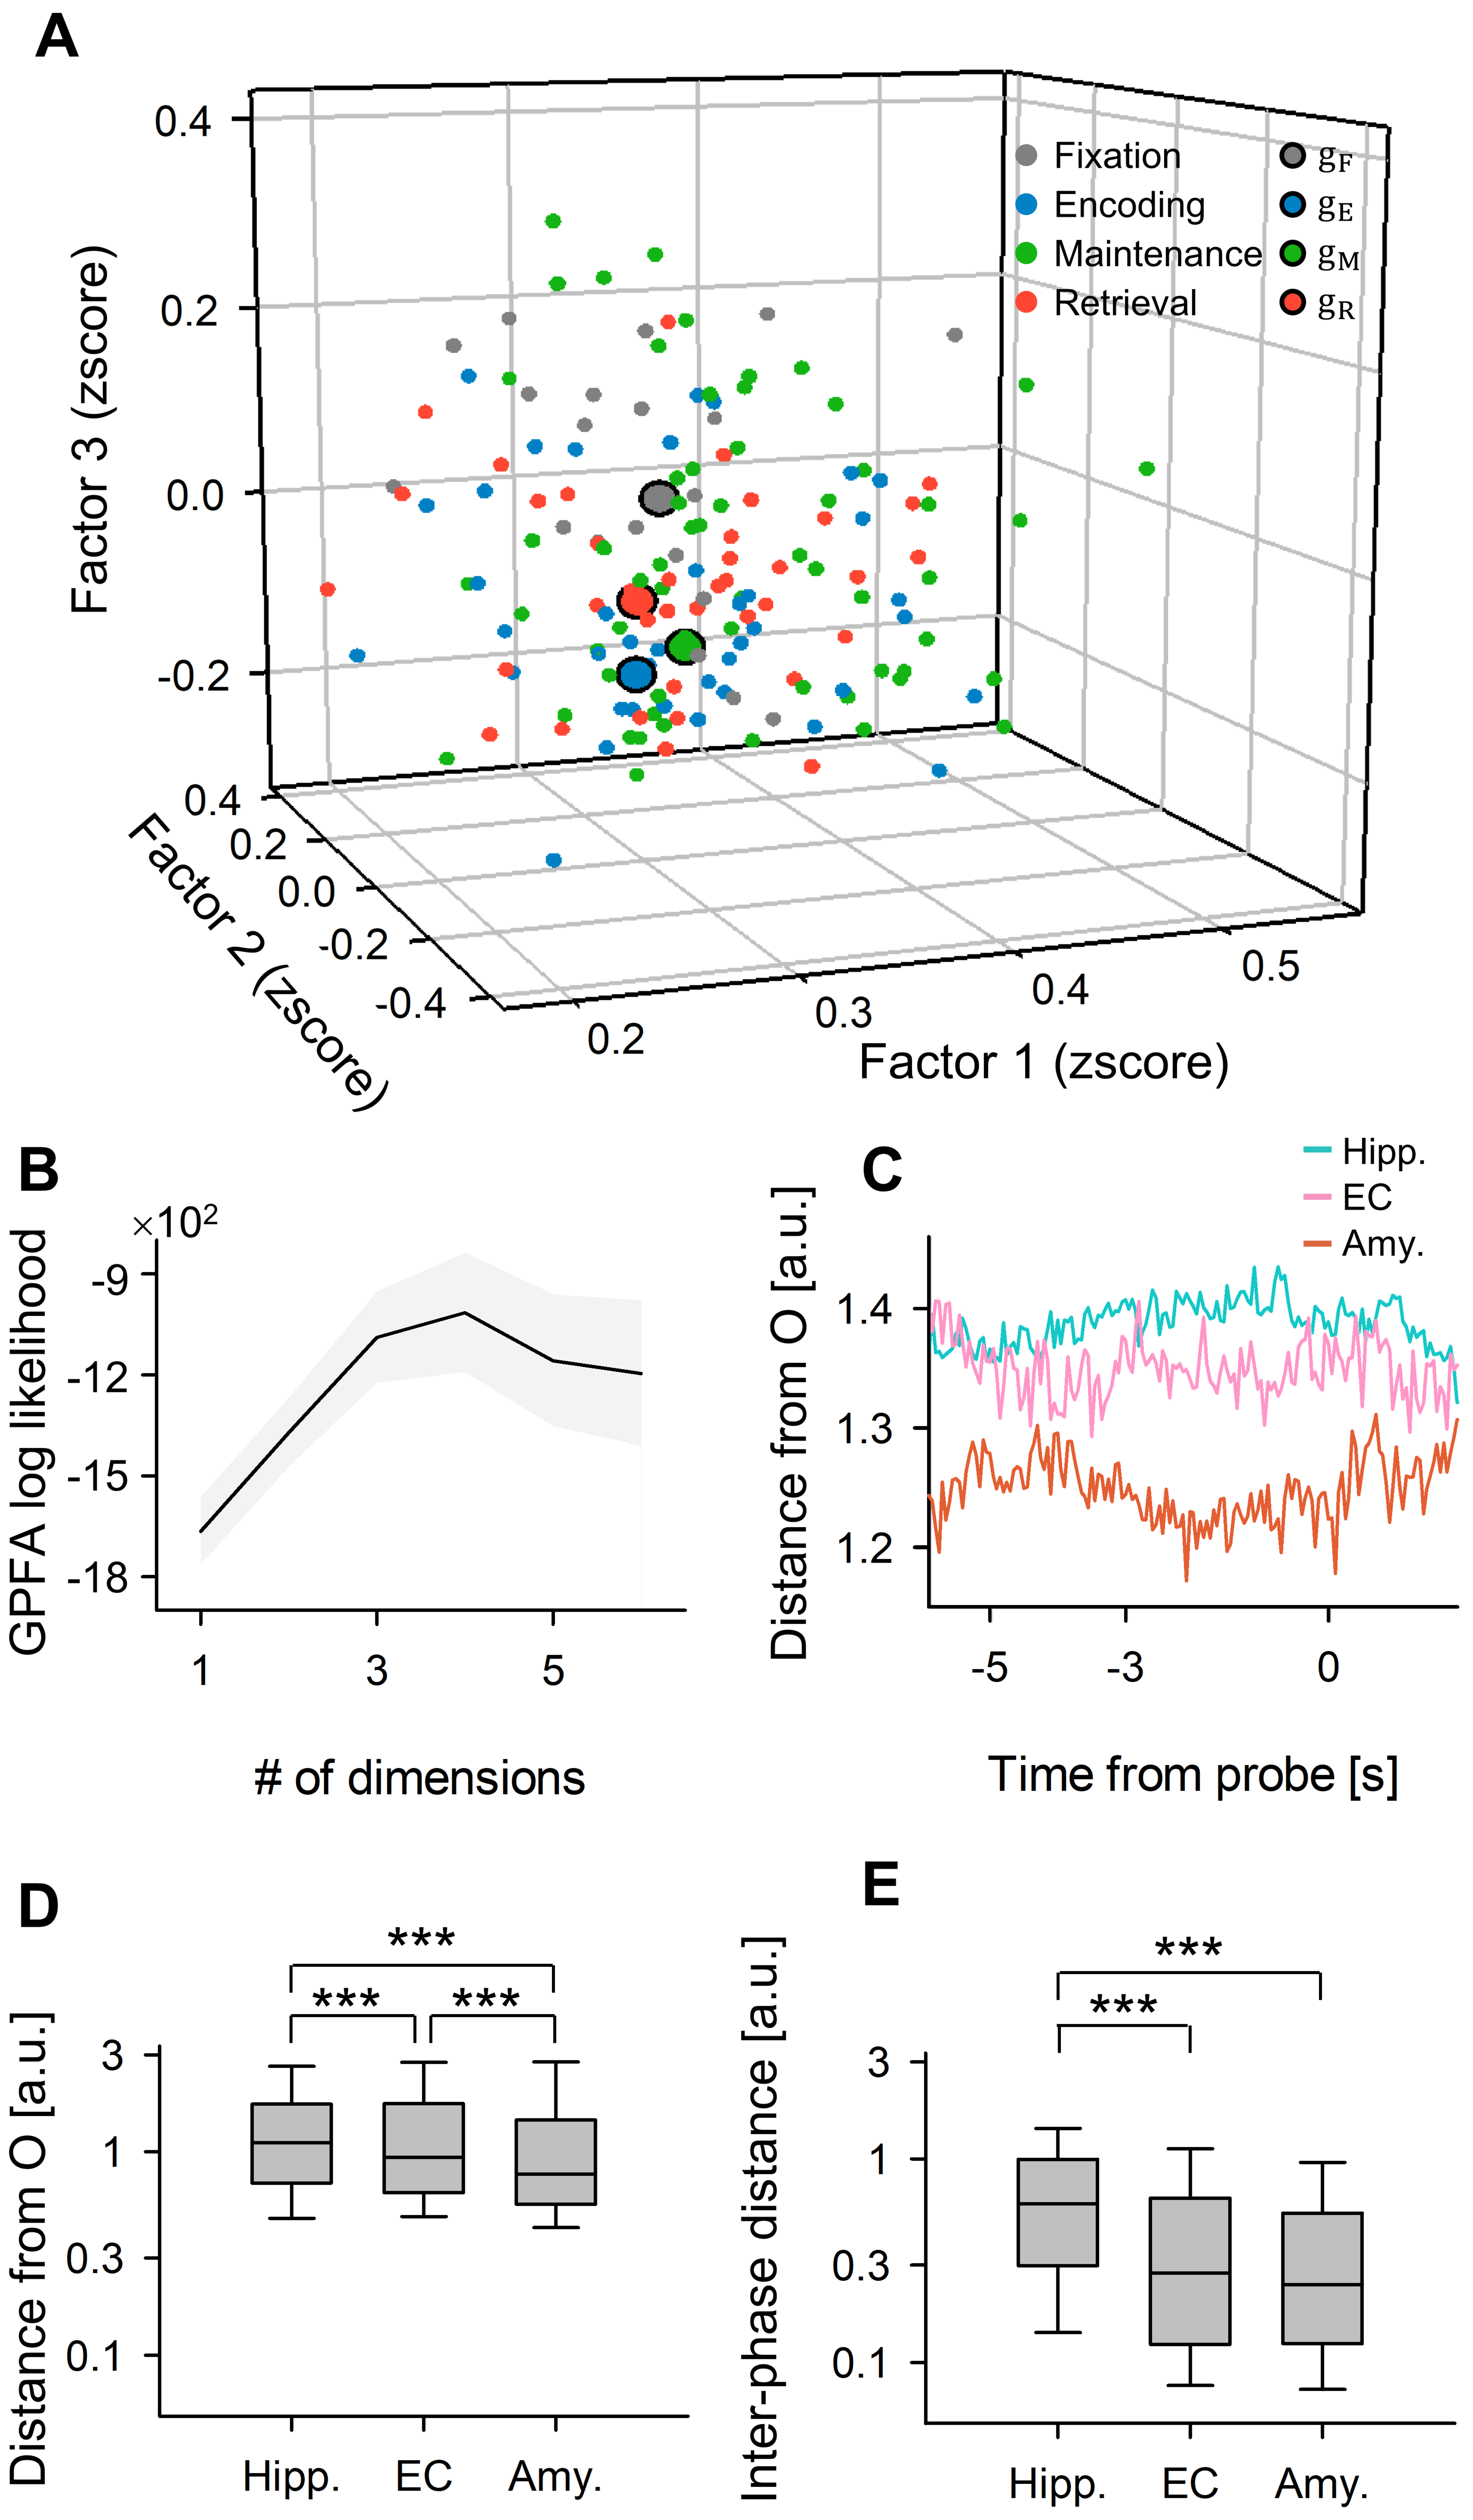
\includegraphics[width=]{./src/figures\GREENENDS /.\GREENSTARTS png/Figure_ID_02.png}
        	\caption{\textbf{
State-dependent hippocampal neural trajectory
}
\smallskip
\\
\textbf{\textit{\GREENENDS A\GREENSTARTS .}} The neural trajectory in the first three-dimensional factors computed using GPFA is illustrated. Smaller dots represent the coordinates of 50-ms neural trajectory bins, while larger dots outlined in \textit{black} denote the geometric medians for subsequent phases in the Sternberg working memory task: fixation (\textit{gray}), encoding (\textit{blue}), maintenance (\textit{green}), and retrieval (\textit{red})\cite{yu\GREENENDS \REDSTARTS ll\REDENDS _\GREENSTARTS gaussian-process_2009}. \textbf{\textit{B.}} This figure demonstrates the log-likelihood of GP\GREENENDS F\GREENSTARTS A models in conjunction with the number of dimensions employed to embed multi-unit spikes in MTL regions. Significantly, the optimal dimension was determined to be three, ascertained through the use of the elbow method\cite{virtanen_scipy_2020}. \textbf{\textit{C.}} In this segment, the distance of neural trajectory is mapped from the origin ($O$) for the hippocampus (Hipp.), entorhinal cortex (EC), and amygdala (Amy.), and is plotted in relation to the time from the probe's commencement\cite{boran_dataset_2020}. \textbf{\textit{D.}} The following graph illustrates the trajectory distance from $O$ within MTL regions, whereby the hippocampus exhibits the greatest distance, succeeded by the EC and the Amygdala\cite{fernandez-ruiz_long-duration_2019}. \textbf{\textit{E.}} The subsequent representation indicates inter-phase trajectory distances within the MTL regions\cite{liu_consensus_2022}.
Abbreviations:
}
        	\label{fig:02}
        \end{figure*}
        \clearpage
        \begin{figure*}[ht]
            \pdfbookmark[2]{ID 03}{figure_id_03}
        	\centering
            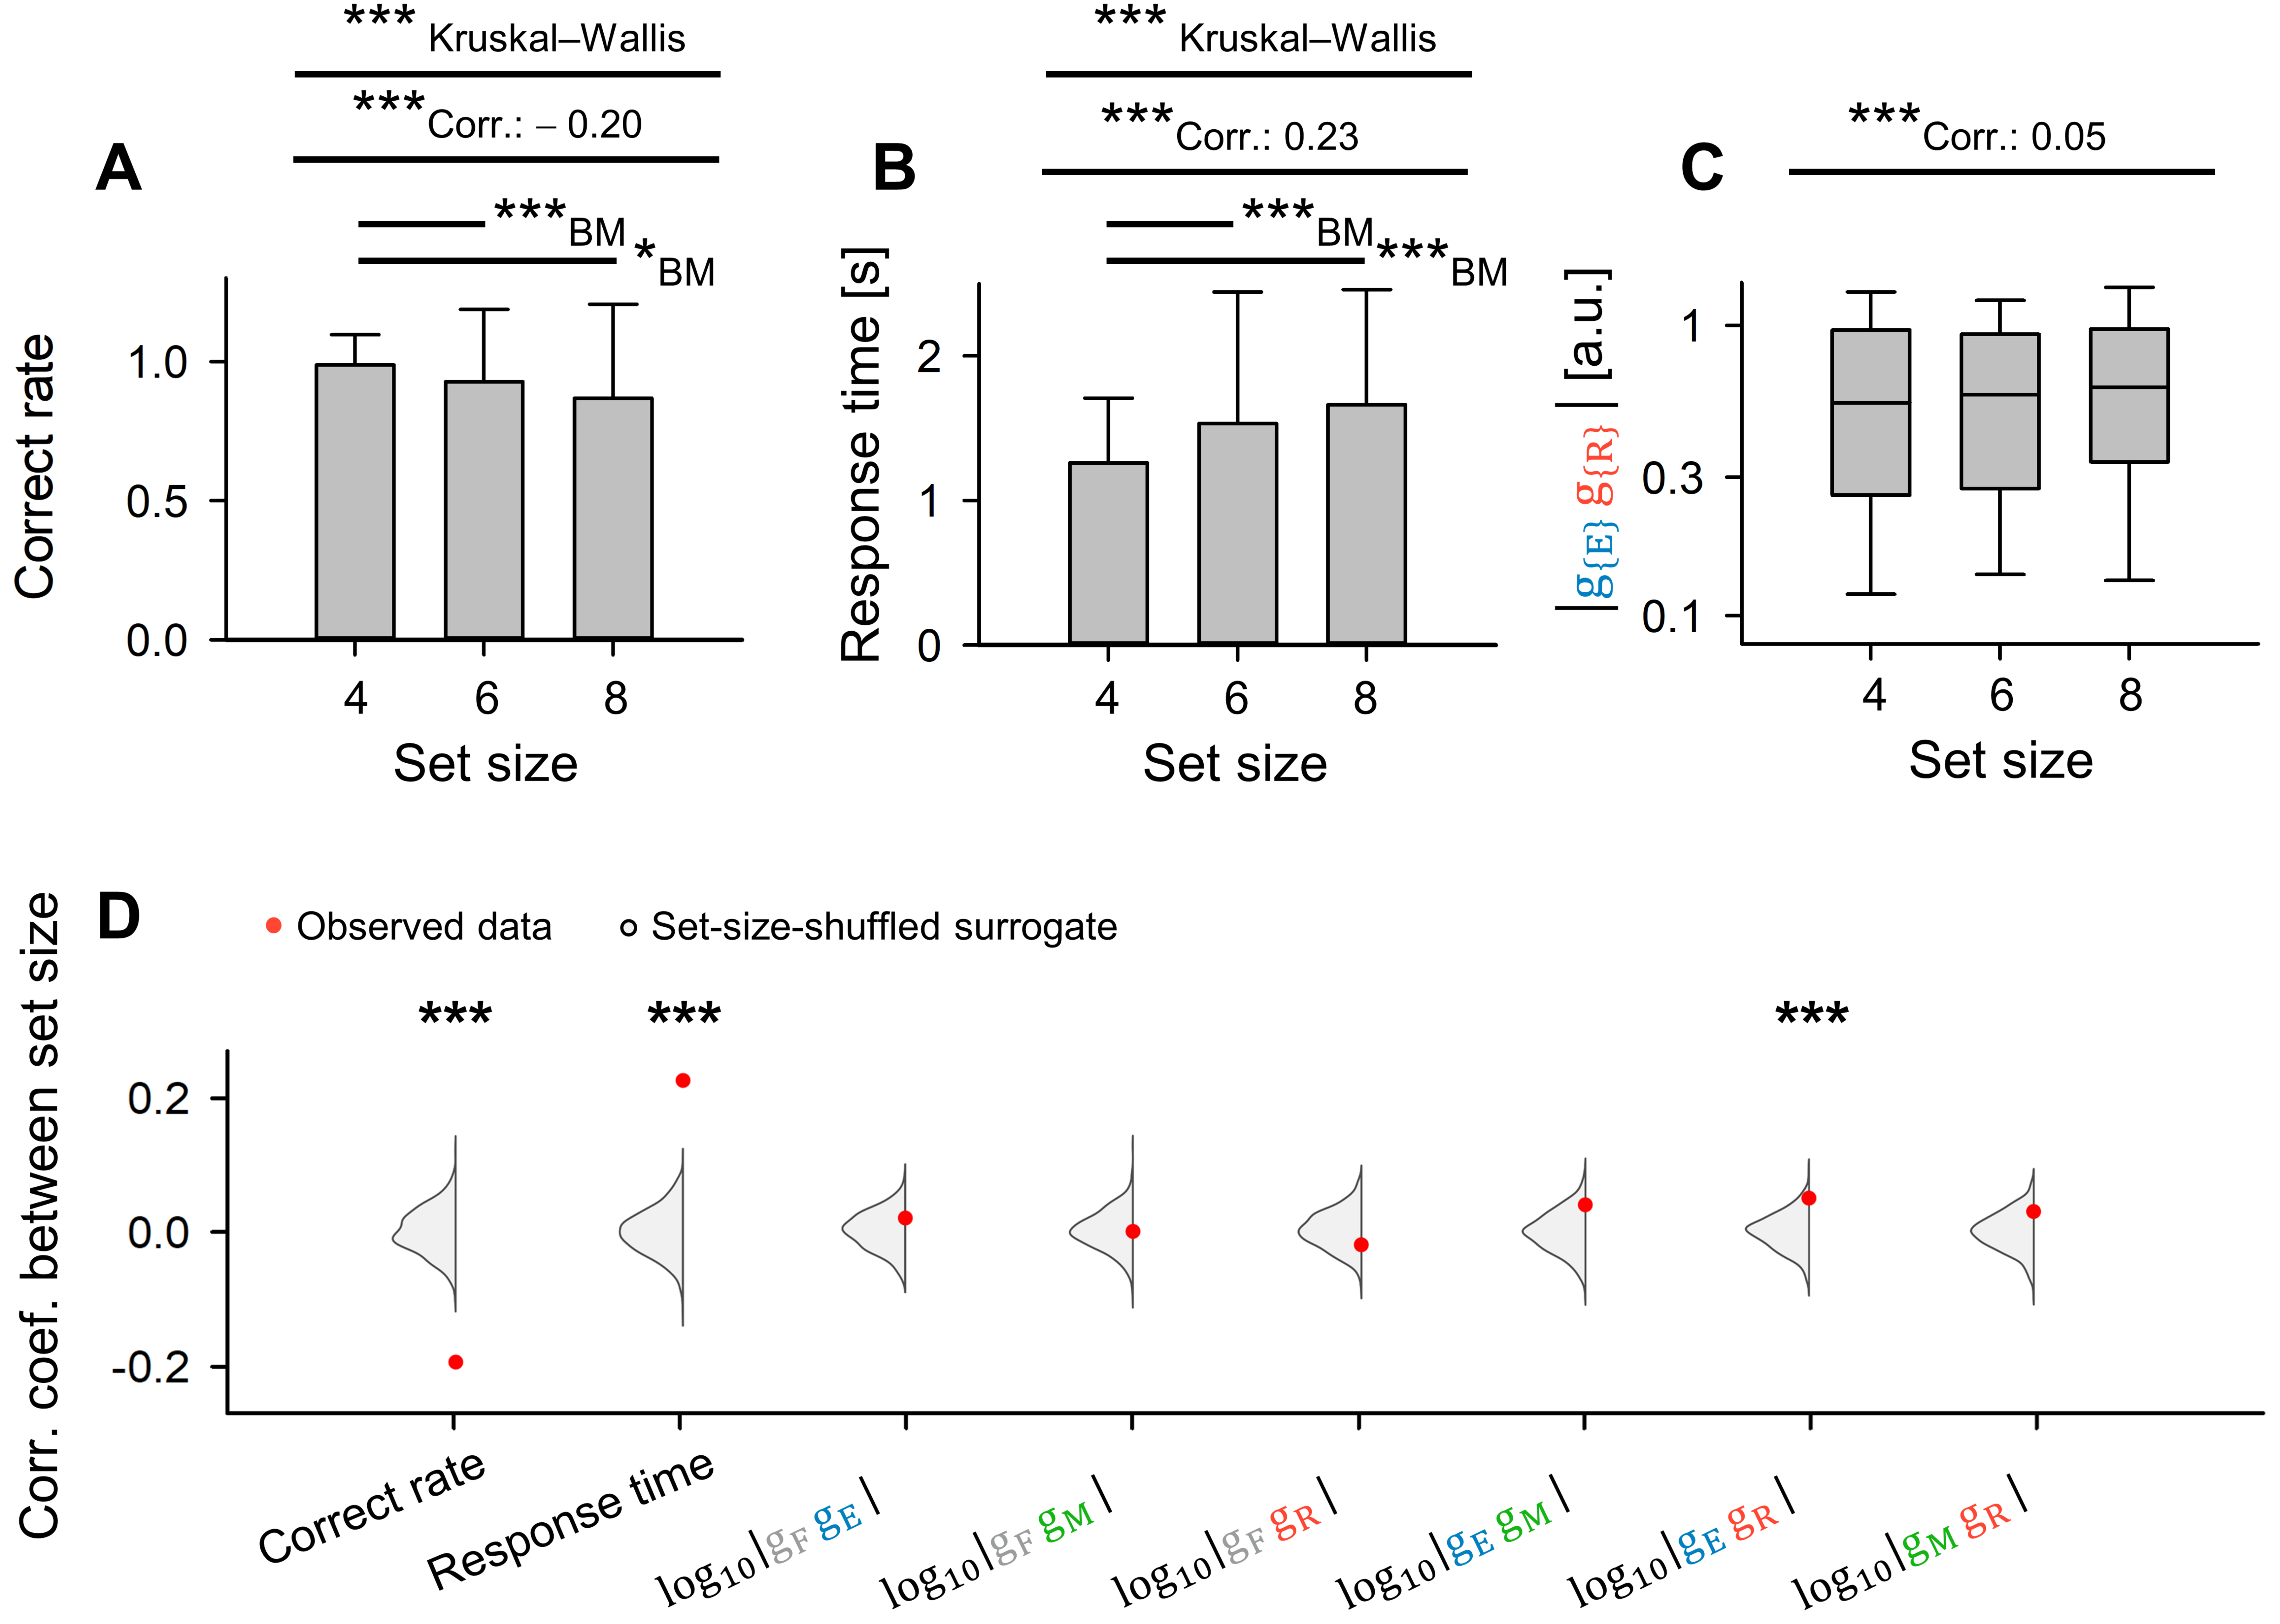
\includegraphics[width=1\textwidth]{./src/figures/.png/Figure_ID_03.png}
        	\caption{\textbf{
Dependence of Trajectory Distance on Memory Load Between Encoding and Retrieval States in the Hippocampus 
}
\smallskip
\\
\textbf{\textit{A.}} Set size (the number of letters to encode) and correct rate in the WM task (coefficient = $-0.20$, ***\textit{p} $<$ 0.001) \cite{van_vugt_hippocampal_2010, li_functional_2023, borders_hippocampus_2022}. \textbf{\textit{B.}} Set size and response time (coefficient = $0.23$, ***\textit{p} $<$ 0.001) \cite{dimakopoulos_information_2022}.  \textbf{\textit{C.}} Set size and the inter-phase distances between encoding and retrieval phases ($\Vert \mathrm{g_{E}g_{R}} \Vert$) (correlation coefficient = 0.05) \cite{li_functional_2023}. \textbf{\textit{D.}} \textit{Red} dots illustrate experimentally observed correlations between set size and the following parameters: correct rate, response time, $\log_{10}{\Vert \mathrm{g_{F}g_{E}} \Vert}$, $\log_{10}{\Vert \mathrm{g_{F}g_{M}} \Vert}$, $\log_{10}{\Vert \mathrm{g_{F}g_{R}} \Vert}$, $\log_{10}{\Vert \mathrm{g_{E}g_{M}} \Vert}$, $\log_{10}{\Vert \mathrm{g_{E}g_{R}} \Vert}$, and $\log_{10}{\Vert \mathrm{g_{M}g_{R}} \Vert}$. The \textit{gray} kernel density plot indicates corresponding set-size-shuffled surrogate (\textit{n} = 1,000) (***\textit{p}s $<$ 0.001) \cite{norimoto_hippocampal_2018, hajos_input-output_2013}.
}
% width=1\textwidth
        	\label{fig:03}
        \end{figure*}
        \clearpage
        \begin{figure*}[ht]
            \pdfbookmark[2]{ID 04}{figure_id_04}
        	\centering
            \includegraphics[width=1\textwidth]{./src/figures/.png/Figure_ID_04.png}
        	\caption{\textbf{
Detection of SWRs in Presumed CA1 Regions
}
\smallskip
\\
\textbf{\textit{A.}} Two-dimensional UMAP (uniform manifold approximation and projection) projection of multiunit spikes during candidates for SWRs (\textit{purple}) and non-SWRs (\textit{yellow})\cite{mcinnes_umap_2018}. \textbf{\textit{B.}}  Cumulative density plot of silhouette scores, utilized as a gauge for UMAP clustering quality, for hippocampal regions (refer to Table~\ref{tab:02}). Lands exceeding a silhouette score of 0.60 (equating to the $75^{th}$ percentile) were classified as probable CA1 regions. Candidates for SWRs and non-SWRs identified in these hypothetical CA1 regions were defined as SWRs and non-SWRs (\textit{n}s = 1,170), respectively\cite{rousseeuw_silhouettes_1987}. \textbf{\textit{C.}}  The distribution of durations for both SWRs (\textit{purple}) and non-SWRs (\textit{yellow}) are congruent, given their definitions (93.0 [65.4] ms, median [IQR])\cite{girardeau_selective_2009}\cite{norman_hippocampal_2021}. \textbf{\textit{D.}}  SWR incidence for SWRs (\textit{purple}) and non-SWRs (\textit{yellow}) over time from probing, represented as a mean value \textpm 95\% confidence interval. Despite their singular character, the intervals may not be visible due to their narrowness. Note that a significant uptake in SWR incidence was perceived during the first 400 ms of the retrieval phase (0.421 [Hz], *\textit{p} < 0.05, bootstrap test)\cite{buzsaki_hippocampal_2015}\cite{ego-stengel_disruption_2010}\cite{fernandez-ruiz_long-duration_2019}. \textbf{\textit{E.}}  The distributions of ripple band peak amplitudes are presented for non-SWRs (\textit{yellow}; 2.37 [0.33] SD of baseline, median [IQR]) and SWRs (\textit{purple}; 3.05 [0.85] SD of baseline, median [IQR]) (***\textit{p} < 0.001, utilizing the Brunner--Munzel test)\cite{norman_hippocampal_2019}\cite{diba_forward_2007}\cite{liu_consensus_2022}.
}
% width=1\textwidth
        	\label{fig:04}
        \end{figure*}
        \clearpage
        \begin{figure*}[ht]
            \pdfbookmark[2]{ID 05}{figure_id_05}
        	\centering
            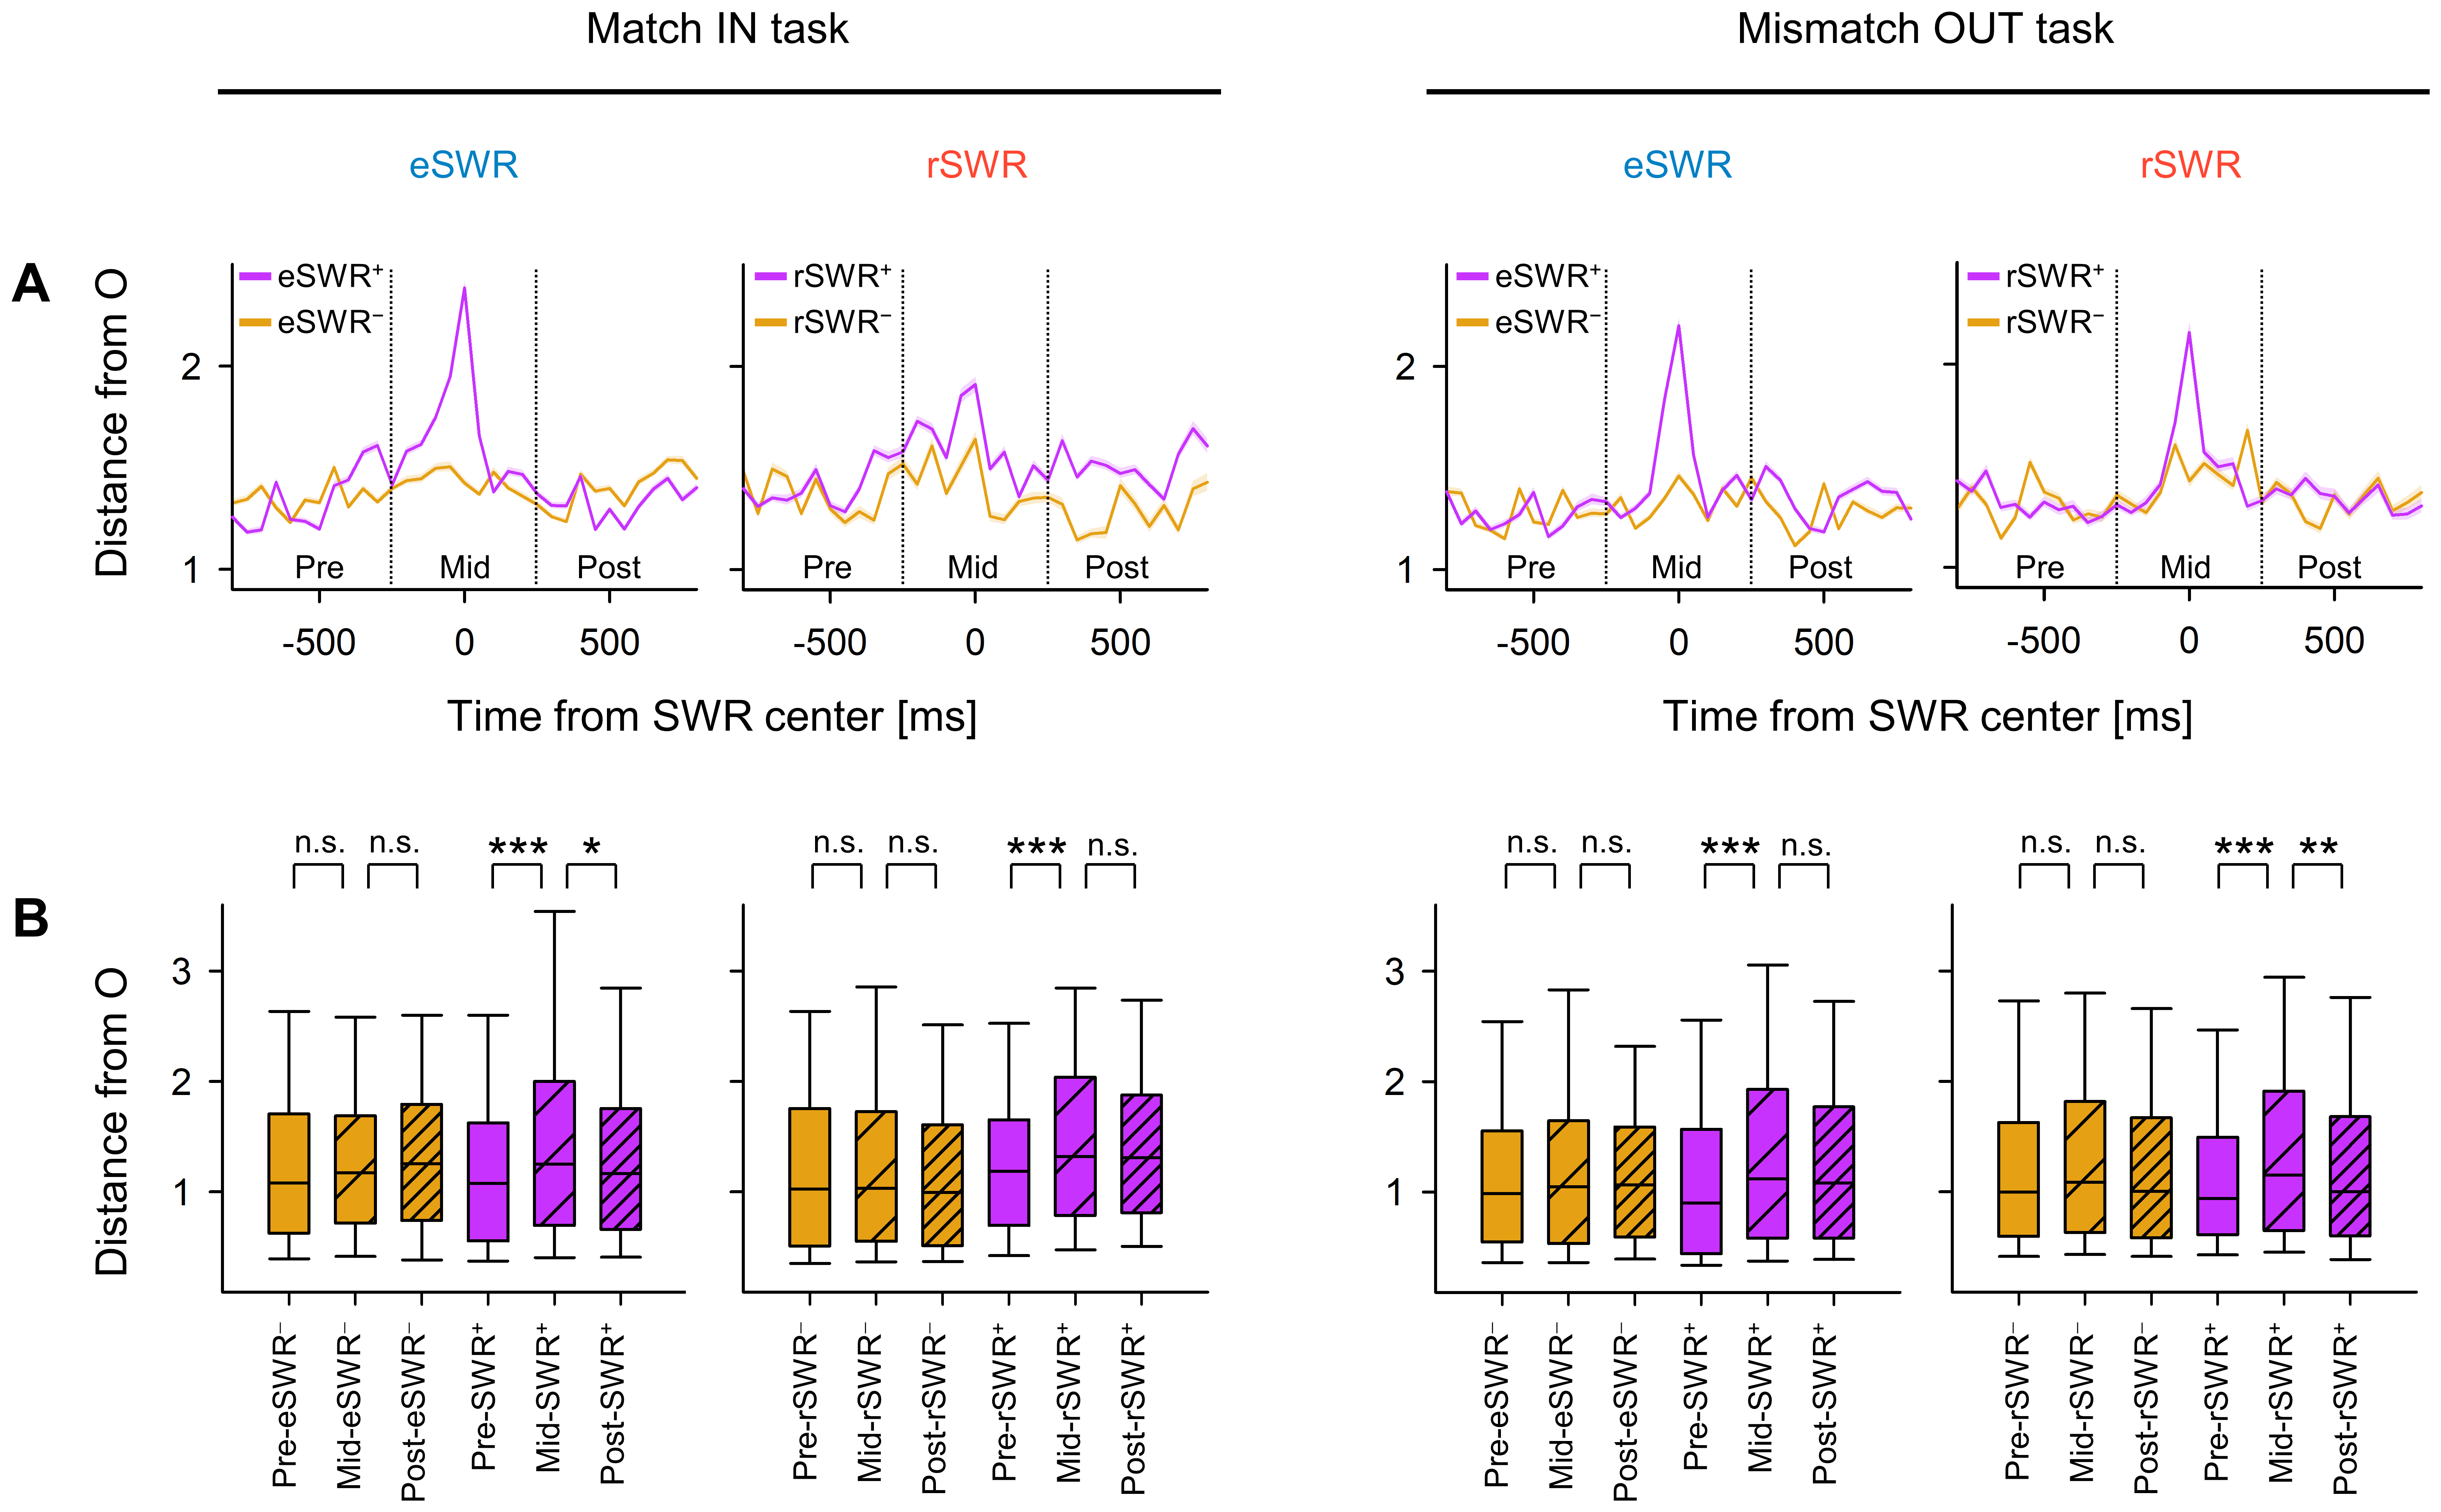
\includegraphics[width=1\textwidth]{./src/figures/.png/Figure_ID_05.png}
        	\caption{\textbf{
Transient Alterations in Neural Trajectory During SWR
}
\smallskip
\\
\textbf{\textit{A.}} Represents the distance from the origin ($O$) of the peri-sharp-wave-ripple (SWR) trajectory expressed as the mean \textpm a 95\% confidence interval, which may not be visible owing to its narrow range \cite{girardeau_selective_2009,norman_hippocampal_2019,buzsaki_hippocampal_2015}. \textbf{\textit{B.}} Illustrates the distance from the origin ($O$) during the pre-, mid-, and post-SWR periods (*\textit{p} $<$ 0.05, **\textit{p} $<$ 0.01, ***\textit{p} $<$ 0.001; according to the Brunner--Munzel test \cite{boran_persistent_2019}). Abbreviations detailed as: SWR, sharp-wave ripple events; eSWR, SWR occurring in the encoding phase; rSWR, SWR happening during the retrieval phase; SWR$^+$, SWR event; SWR$^-$, control events for SWR$^+$; pre-, mid-, or post-SWR, the time intervals from $-800$ to $-250$ ms, from $-250$ to $+250$ ms, or from $+250$ to $+800$ ms, each relative to the SWR center.
}
% width=1\textwidth
        	\label{fig:05}
        \end{figure*}
        \clearpage
        \begin{figure*}[ht]
            \pdfbookmark[2]{ID 06}{figure_id_06}
        	\centering
            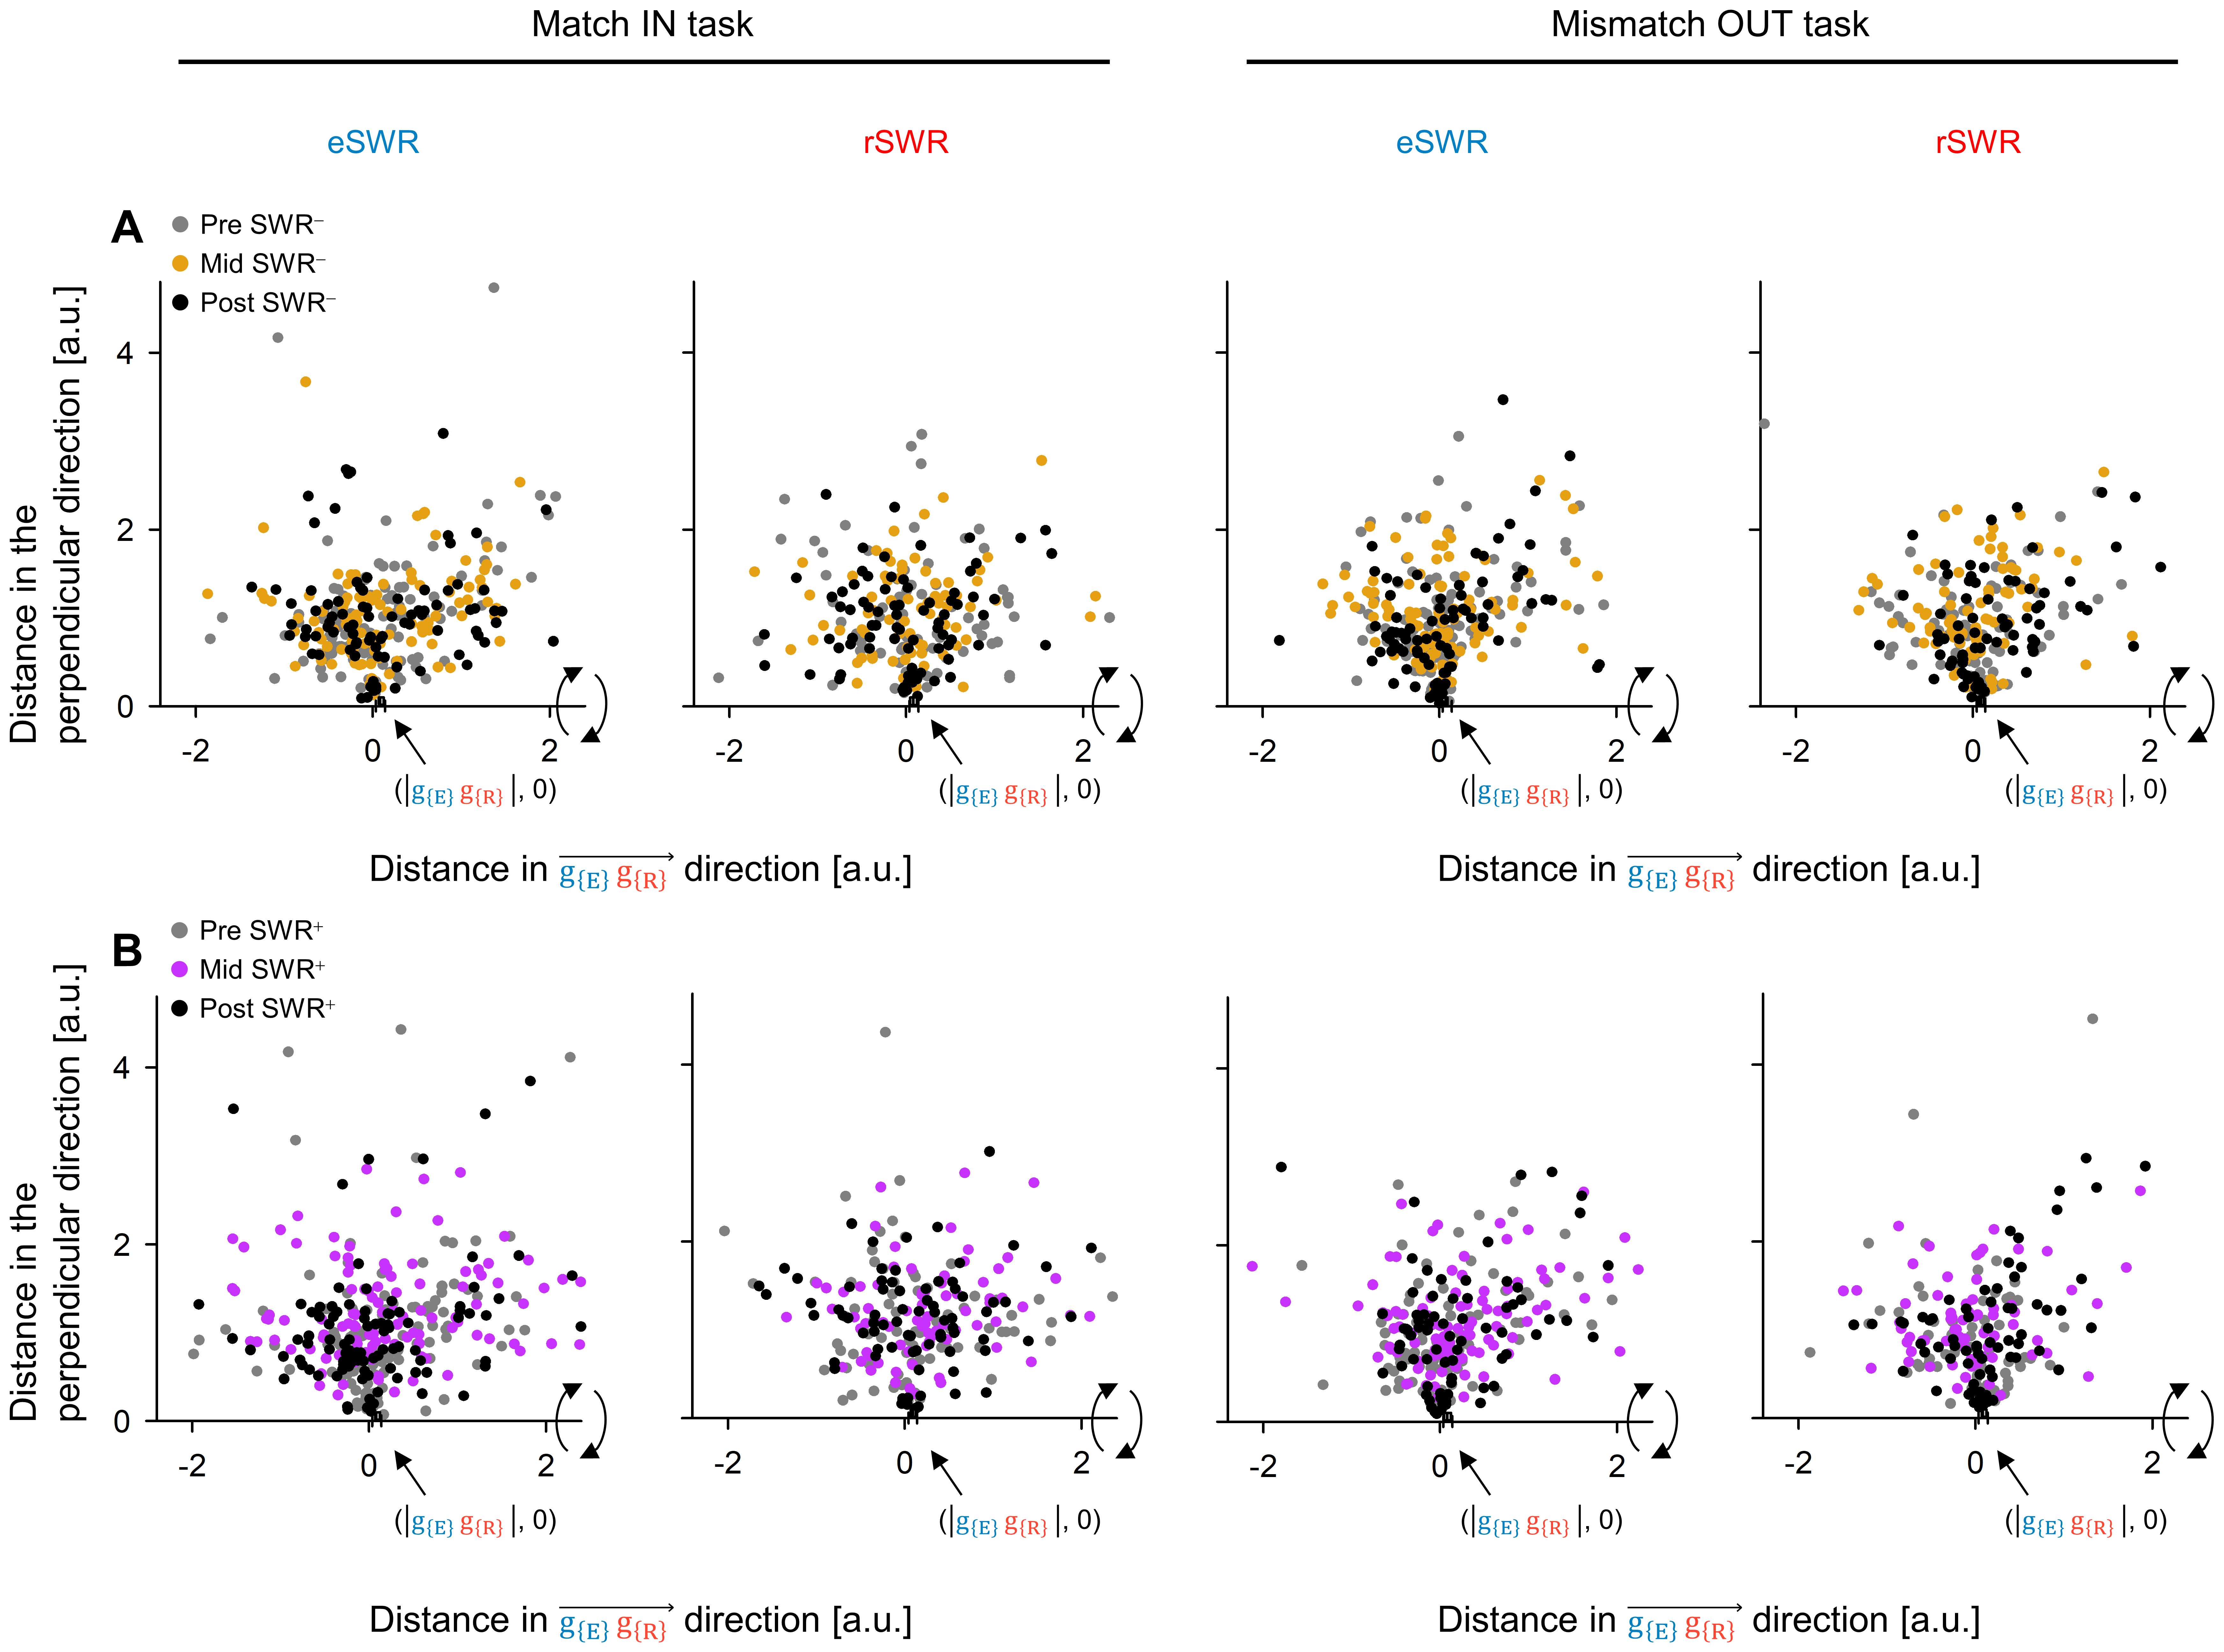
\includegraphics[width=1\textwidth]{./src/figures/.png/Figure_ID_06.png}
        	\caption{\textbf{
Visualization of Neural Trajectory During SWR in Two-Dimensional Space
}
\smallskip
\\
Featured are neural trajectories within the hippocampus during Sharp-Wave Ripple (SWR) events, represented in a two-dimensional space. \textbf{\textit{A.}} Trajectories during pre- (\textit{gray}), mid- (\textit{yellow}), and post-SWR$^-$ (\textit{black}) phases of an SWR event~\cite{buzsaki_hippocampal_2015}. \textbf{\textit{B.}} Corresponding trajectories for SWR$^+$ scenarios as opposed to SWR$^-$~\cite{fernandez-ruiz_long-duration_2019}. The magnitude of $\lVert \mathrm{g_{E}g_{R}} \rVert$ fluctuates within sessions~\cite{liu_consensus_2022}. The projection protocol went as follows: initially, $\mathrm{g_{E}}$ was placed at the origin $O$ (0,0), and $\mathrm{g_{R}}$ at ($\lVert \mathrm{g_{E}g_{R}} \rVert$, 0) via linear transformation~\cite{kim_corticalhippocampal_2022}. Subsequently, the point cloud was rotated around the $\mathrm{g_{E}g_{R}}$ axis (the x-axis) for compatibility with a two-dimensional environment~\cite{yu_gaussian-process_2009}. Consequently, both the distances from $O$ and the angles with respect to the $\mathrm{g_{E}g_{R}}$ axis were kept intact from their original three-dimensional arrangement~\cite{mcinnes_umap_2018}. Abbreviations: SWR denotes Sharp-Wave Ripple events; eSWR refers to SWR during the encoding phase; rSWR indicates SWR during the retrieval phase; SWR$^+$ represents an SWR event; SWR$^-$ designates the control events for SWR$^+$; pre-SWR, mid-SWR, or post-SWR specify the time interval from $-800$ to $-250$ ms, from $-250$ to $+250$ ms, or from $+250$ to $+800$ ms from the center of the SWR respectively~\cite{zhang_hippocampal_2022}.
}
% width=1\textwidth
        	\label{fig:06}
        \end{figure*}
        \clearpage
        \begin{figure*}[ht]
            \pdfbookmark[2]{ID 07}{figure_id_07}
        	\centering
            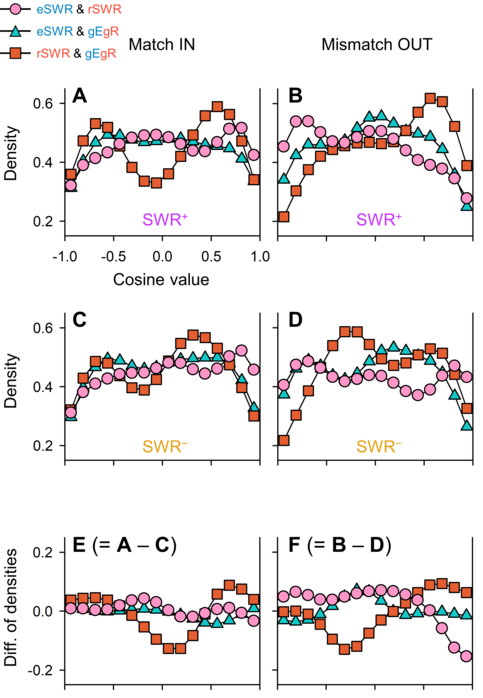
\includegraphics[width=0.5\textwidth]{./src/figures/.png/Figure_ID_07.png}
        	\caption{\textbf{
Neural Trajectory Directions of SWR based on Encoding and Retrieval States
}
\smallskip
\\
\textbf{\textit{A--B}} Kernel Density Estimation (KDE) distribution of $\protect\overrightarrow{{\mathrm{eSWR^+}}} \cdot \protect\overrightarrow{{\mathrm{rSWR^+}}}$ (\textit{pink circles}), $\protect\overrightarrow{{\mathrm{eSWR^+}}} \cdot \protect\overrightarrow{{\mathrm{g_{E}g_{R}}}}$ (\textit{blue triangles}), and $\protect\overrightarrow{{\mathrm{rSWR^+}}} \cdot \protect\overrightarrow{{\mathrm{g_{E}g_{R}}}}$ (\textit{red rectangles}) in Match IN (\textit{A}) and Mismatch OUT tasks (\textit{B})~\cite{li_functional_2023}. \textbf{\textit{C--D}} The corresponding distributions of $\mathrm{SWR^-}$ replace those of $\mathrm{SWR^+}$ in \textit{A--B}~\cite{dimakopoulos_information_2022}. \textbf{\textit{E--F}} The differences in distributions of $\mathrm{SWR^+}$ and $\mathrm{SWR^-}$, emphasizing the SWR components (\textit{E} = \textit{C} $-$ \textit{A}; \textit{F} = \textit{B} $-$ \textit{D}). Notice the biphasic distributions of $\protect\overrightarrow{{\mathrm{rSWR^-}}} \cdot \protect\overrightarrow{{\mathrm{g_{E}g_{R}}}}$, underscoring neural fluctuations between encoding and retrieval states during the Sternberg task~\cite{borders_hippocampus_2022}. Conversely, in the Mismatch OUT task, inverse directionality between $\protect\overrightarrow{{\mathrm{eSWR^+}}}$ and $\protect\overrightarrow{{\mathrm{rSWR^+}}}$ (\textit{pink circles}) was identified, but not in the Match IN task (\textbf{\textit{E--F}})~\cite{naber_reciprocal_2001,van_strien_anatomy_2009}. Lastly, transitions from retrieval to encoding states were observed for the SWR components in both Match IN and Mismatch OUT tasks (\textit{red rectangles} in \textit{E--F})~\cite{niediek_reliable_2016,schomburg_spiking_2012}.
}
% width=0.5\textwidth
        	\label{fig:07}
        \end{figure*\GREENENDS \REDSTARTS igures\REDENDS }


%%%%%%%%%%%%%%%%%%%%%%%%%%%%%%%%%%%%%%%%%%%%%%%%%%%%%%%%%%%%%%%%%%%%%%%%%%%%%%%%
%% END
%%%%%%%%%%%%%%%%%%%%%%%%%%%%%%%%%%%%%%%%%%%%%%%%%%%%%%%%%%%%%%%%%%%%%%%%%%%%%%%%

\end{document}
\REDSTARTS \endinput\REDENDS 
